% The Mathematics and Algorithms of Texas Hold'em Poker
% Author: Cathy Li — compiled with Tectonic
\documentclass[11pt,a4paper]{article}

\usepackage{amsmath}
\usepackage{amssymb}
\usepackage{amsthm}
\usepackage{graphicx}
\usepackage{xcolor}
\usepackage{geometry}
\usepackage{booktabs}
\usepackage{tabularx}
\usepackage{adjustbox}
\usepackage{enumitem}
\usepackage{needspace}
\usepackage[ruled,vlined,linesnumbered]{algorithm2e}
\usepackage{tikz}
\usetikzlibrary{arrows.meta,positioning}
\usepackage{fancyhdr}

% hyperref ALWAYS last among content packages
\usepackage[
    colorlinks=true,
    linkcolor=linknavy,
    citecolor=darkgray,
    urlcolor=linknavy,
    bookmarks=true,
    bookmarksnumbered=true,
    unicode=true
]{hyperref}

\geometry{a4paper, top=2.5cm, bottom=2.5cm, left=2.5cm, right=2.5cm}

% Orphan/widow control
\widowpenalty=10000
\clubpenalty=10000

% Allow slightly stretched interword spacing instead of overfull lines
\setlength{\emergencystretch}{3em}

\definecolor{linknavy}{RGB}{28,62,95}
\definecolor{accent}{RGB}{46,93,78}
\definecolor{boxbg}{RGB}{240,244,242}
\definecolor{rulegray}{RGB}{120,120,120}

% Theorem environments
\theoremstyle{plain}
\newtheorem{theorem}{Theorem}[section]
\newtheorem{lemma}[theorem]{Lemma}
\newtheorem{proposition}[theorem]{Proposition}
\theoremstyle{definition}
\newtheorem{definition}{Definition}[section]
\newtheorem{example}{Example}[section]
\theoremstyle{remark}
\newtheorem{remark}{Remark}[section]

% Algorithm styling
\SetAlFnt{\small}
\SetAlCapFnt{\small}
\SetAlCapNameFnt{\small}

% Caption and float separation: captions, tables, and figures must sit
% clearly off the surrounding text and off each other
\setlength{\abovecaptionskip}{12pt}
\setlength{\belowcaptionskip}{16pt}
\setlength{\textfloatsep}{26pt plus 4pt minus 2pt}
\setlength{\intextsep}{24pt plus 4pt minus 2pt}
\setlength{\floatsep}{18pt plus 2pt minus 2pt}
% Airier table rows
\renewcommand{\arraystretch}{1.22}

\makeatletter
% Float pages: content starts at the top of the page (no vertical centering),
% fixed separation between stacked floats, leftover space at the bottom.
\setlength{\@fptop}{0pt}
\setlength{\@fpsep}{24pt}
\setlength{\@fpbot}{0pt plus 1fil}
\makeatother

% Footer with an author stamp so the compiled document is always
% identifiable on every page (page number on the right).
\pagestyle{fancy}
\fancyhf{}
\fancyfoot[L]{\footnotesize\color{rulegray}Cathy Li \textperiodcentered\ September 14, 2026}
\fancyfoot[R]{\footnotesize\thepage}
\renewcommand{\headrulewidth}{0pt}
\renewcommand{\footrulewidth}{0pt}
\setlength{\footskip}{32pt}

% Compact quotation of inline math operators
\DeclareMathOperator{\E}{\mathbb{E}}
\DeclareMathOperator{\Var}{\mathrm{Var}}
\DeclareMathOperator{\SE}{\mathrm{SE}}
\DeclareMathOperator{\br}{\mathrm{BR}}
\newcommand{\eq}{e}

\hypersetup{
    pdftitle={The Mathematics and Algorithms of Texas Hold'em Poker: From Card Probabilities to Superhuman Play},
    pdfauthor={Cathy Li},
    pdfsubject={Game theory, artificial intelligence, and probability in poker},
    pdfkeywords={Texas Hold'em, poker, Nash equilibrium, counterfactual regret minimization, Monte Carlo, reinforcement learning, game theory}
}

\begin{document}

% ============ Title block (no cover page) ============
\begin{center}
    {\LARGE\bfseries The Mathematics and Algorithms of\\[2pt] Texas Hold'em Poker\par}
    \vspace{6pt}
    {\large From Card Probabilities to Superhuman Play\par}
    \vspace{14pt}
    {\normalsize Cathy Li\par}
    \vspace{4pt}
    {\small September 2026\par}
    \vspace{10pt}
    {\color{rulegray}\rule{0.72\textwidth}{0.5pt}\par}
\end{center}
\vspace{4pt}

\begin{abstract}
\noindent
Texas Hold'em is the most strategically rich form of poker played at scale and, for the same reason, has served for three decades as the canonical testbed for decision making under uncertainty. This paper presents a self-contained treatment of the mathematical and algorithmic principles that underpin strong play. We begin with the combinatorial and probabilistic foundations of the game: hand frequencies, equity, pot odds, expected value, and the variance structure that dominates short-term results. We then develop the algorithmic toolkit in increasing order of sophistication: rule-based expert systems driven by hand strength, position, and pot odds; Monte Carlo equity estimators whose accuracy decays as $1/\sqrt{n}$; game-theoretic formulations of imperfect-information games in extensive form; counterfactual regret minimization (CFR) and its sampling and function-approximation variants, including CFR$+$ and Deep CFR; and reinforcement-learning approaches culminating in the superhuman systems DeepStack, Libratus, and Pluribus. We accompany the theory with a concrete implementation---a No-Limit Hold'em engine with five AI paradigms sharing one table---and report a 100{,}000-hand simulation study quantifying how the paradigms' win rates, aggression, and showdown statistics differ in practice. Throughout, emphasis is placed on rigorous statements, convergence guarantees, and the engineering compromises---state abstraction, action abstraction, and equilibrium approximation---that make theory tractable in a game whose full tree contains more game states than there are atoms in the observable universe.
\end{abstract}

\vspace{2pt}
\noindent\textbf{Keywords:} Texas Hold'em; imperfect-information games; Nash equilibrium; counterfactual regret minimization; Monte Carlo methods; reinforcement learning; abstraction.

\vspace{8pt}
{\small\tableofcontents}
\clearpage

% !TeX root = ../main.tex
\section{Introduction}\label{sec:intro}

Poker occupies a unique position at the intersection of probability theory, game theory, and artificial intelligence. Unlike chess or Go, it is a game of \emph{imperfect information}: each player sees only a fragment of the true state, and the deliberate concealment of cards creates strategic phenomena---bluffing, trapping, and the delicate balance between exploiting weak opponents and remaining unexploitable oneself---that have no analogue in perfect-information games. It is also a game of chance at the level of a single hand yet a game of skill in the long run, a duality that makes it an ideal laboratory for studying decision making under uncertainty. These properties led the artificial intelligence community to adopt Texas Hold'em, the most popular variant, as a benchmark of progressively increasing difficulty: first the limit (fixed-bet) heads-up form, then no-limit heads-up, and finally no-limit multiplayer games against several simultaneous opponents.

The scientific arc of this program is remarkably complete. Early systems of the 1990s and 2000s relied on hand-crafted expert knowledge and opponent modeling~\cite{billings2002challenge}. The arrival of \emph{counterfactual regret minimization} (CFR) in 2007 provided the first practical algorithm for approximating Nash equilibria in enormous imperfect-information games~\cite{zinkevich2007regret}, and by 2015 the Cepheus project had essentially solved heads-up limit Hold'em~\cite{bowling2015ceph}. In 2017 two independent systems, DeepStack~\cite{moravcik2017deepstack} and Libratus~\cite{brown2017libratus}, defeated human professionals in heads-up no-limit Hold'em---the game tree of which contains roughly $10^{160}$ decision points~\cite{sandholm2015abstraction}. Two years later Pluribus extended superhuman play to six-player no-limit Hold'em~\cite{brown2019pluribus}, a setting where the very notion of a unique optimal strategy dissolves and agents must instead target robust, unexploitable policies.

This paper is written for readers who want both the mathematics and the algorithms in one place, at full rigor but without unexplained leaps. Three goals organise the presentation. First, we build the probabilistic core that any strong player or program must internalize: hand combinatorics (Section~\ref{sec:probability}), equity and pot odds, expected value, and the variance that governs bankroll requirements. Second, we develop the algorithmic ladder in order of conceptual depth: rule-based expert systems and Monte Carlo estimation (Section~\ref{sec:evaluation}), the extensive-form game-theoretic framework (Section~\ref{sec:gametheory}), regret minimization and CFR with its modern variants (Section~\ref{sec:cfr}), and reinforcement learning in imperfect-information settings, including the architectures of DeepStack, Libratus, and Pluribus (Section~\ref{sec:rl}). Third, we ground the entire discussion in a working implementation: a strictly rule-compliant No-Limit Hold'em engine with five AI paradigms at one table, which we use in Section~\ref{sec:experiments} to quantify---via a 100{,}000-hand simulation---how abstract theory translates into observable differences in win rate and playing style.

The paper is deliberately self-contained. Every algorithm described is either derived from first principles or accompanied by pseudocode faithful to a working implementation; every probabilistic claim is either proved or reducible to a one-line application of a stated theorem. Where a rigorous treatment would require measure-theoretic machinery---for instance, the full generality of stochastic games---we restrict attention to the finite structures that Hold'em actually presents, which suffice for every result we state. Readers interested primarily in the practical study can jump directly to Section~\ref{sec:experiments} after Sections~\ref{sec:gametheory} and~\ref{sec:cfr}, on which the experimental agents' designs rest.

\section{The Game of Texas Hold'em}\label{sec:game}

\subsection{Structure and terminology}

Texas Hold'em is played with a standard 52-card deck. Each player receives two private \emph{hole cards}; five \emph{community cards} are dealt face up in stages and shared by all players. A hand consists of four betting rounds interleaved with the card deals: \emph{preflop} (hole cards dealt), \emph{flop} (three community cards), \emph{turn} (one card), and \emph{river} (one final card). At the end of each hand, remaining players form their best five-card poker hand from the seven available cards (two hole plus five community); the player with the highest-ranked hand wins the pot, or the pot is split among tied players.

In the no-limit variant, at each decision a player may fold (surrender the hand and any chips already wagered), check or call (match the current wager, or pass if no wager is pending), or raise to any amount between a minimum raise size and the player's entire remaining stack. Two forced wagers seed the pot: the \emph{small blind} and \emph{big blind}, posted before the cards are dealt by the two seats to the left of a \emph{dealer button} that rotates one seat each hand. The minimum raise equals the size of the last raise or bet; a raise of less than the minimum is permitted only when it exhausts a player's stack (a \emph{short all-in}), in which case betting is not reopened for players who have already acted.

Figure~\ref{fig:streets} summarises the flow of a hand. Two details of correct rule enforcement deserve emphasis because naive implementations routinely botch them. First, when players are all-in and no further betting is possible, the remaining community cards are dealt and the hand proceeds directly to showdown, frequently producing layered \emph{side pots}: a player can only win a share of the pot proportional to the amount they actually matched from each opponent. Second, the preflop round is closed by an option for the big blind: if every other player has merely called, the big blind may still raise, because posting the blind is not a voluntary action.

\begin{figure}[htbp]
\centering
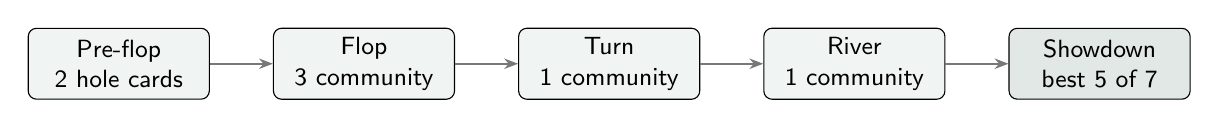
\begin{tikzpicture}[
  stage/.style={draw, rounded corners=3pt, minimum width=2.3cm, minimum height=0.9cm,
                align=center, font=\small\sffamily, fill=boxbg},
  arr/.style={-{Stealth[length=5pt]}, thick, rulegray}
]
  \node[stage] (pre) {Pre-flop\\2 hole cards};
  \node[stage, right=0.8cm of pre] (flop) {Flop\\3 community};
  \node[stage, right=0.8cm of flop] (turn) {Turn\\1 community};
  \node[stage, right=0.8cm of turn] (riv) {River\\1 community};
  \node[stage, right=0.8cm of riv, fill=accent!14] (sd) {Showdown\\best 5 of 7};
  \draw[arr] (pre) -- (flop);
  \draw[arr] (flop) -- (turn);
  \draw[arr] (turn) -- (riv);
  \draw[arr] (riv) -- (sd);
\end{tikzpicture}
\caption{The four betting streets of a Texas Hold'em hand. Each street ends when all active players have matched the largest wager or are all-in; a hand may terminate prematurely by folds at any point, in which case the last remaining player takes the pot without showdown.}
\label{fig:streets}
\end{figure}

\subsection{Hand rankings}\label{sec:rankings}

Five-card hands are ranked in nine categories, each compared within itself by kickers: straight flush (five consecutive cards of one suit, an ace-high straight flush being the \emph{royal flush}), four of a kind, full house (three of a kind plus a pair), flush, straight, three of a kind, two pair, one pair, and high card. The ranking is not arbitrary: as Section~\ref{sec:probability} quantifies, it reflects the number of card combinations that realise each category, so that rarer categories beat common ones with near-total reliability across the opponent's distribution of holdings.

\subsection{From cards to decisions}

A single hand of Hold'em presents each player with only a handful of decision points---at minimum one per street, plus extra decisions for each raise cycle---yet the state space is astronomical. Heads-up no-limit Hold'em has on the order of $10^{160}$ decision points when stack-to-pot ratios allow deep betting trees~\cite{sandholm2015abstraction}, and even the limit variant contains $10^{18}$ game states. Consequently, every practical algorithm in this paper couples a search, estimation, or learning procedure with an \emph{abstraction} that compresses the state space to a tractable size. The art of poker AI is largely the art of designing abstractions whose equilibria are close to equilibria of the real game---a theme developed quantitatively in Sections~\ref{sec:cfr} and~\ref{sec:experiments}.

% !TeX root = ../main.tex
\section{Probability Foundations}\label{sec:probability}

\subsection{Combinatorics of the deck}

All card probabilities flow from one primitive: the number of ways to choose $k$ unordered cards from $n$ distinct cards,
\begin{equation}\label{eq:binom}
\binom{n}{k} \;=\; \frac{n!}{k!\,(n-k)!},
\end{equation}
because every hand in poker is an unordered subset of the deck, and (before any cards are observed) all subsets are equiprobable. Texas Hold'em uses the $k=2$ and $k=5$ cases at the moment cards are assigned to players, and the $k=7$ case at showdown, where the player's effective hand is the \emph{best five-card subset} of the seven available cards.

The number of distinct starting hands is
\begin{equation}
\binom{52}{2} = \frac{52 \cdot 51}{2} = 1326 .
\end{equation}
Suits are strategically interchangeable, so many holdings are equivalent up to suit isomorphism: there are $13$ pocket pairs, $\binom{13}{2}=78$ suited combinations and $78$ offsuit non-pair combinations, giving $169$ \emph{canonical} starting hands. A specific pair such as $Q\spadesuit Q\heartsuit$ has probability $6/1326$ (six suit pairings), a specific suited hand such as $A\spadesuit K\spadesuit$ has probability $4/1326$, and a specific offsuit hand such as $A\spadesuit K\heartsuit$ has probability $12/1326$. These are the weights one must use when aggregating over the canonical classes.

\subsection{Hand-category frequencies}

Table~\ref{tab:ranks} lists the exact number of five-card and seven-card combinations falling into each ranking category, together with the resulting probabilities. The five-card column is a classical computation; we illustrate with two categories and note that the rest follow the same bookkeeping. For a flush, choose the suit ($4$ ways), then choose $5$ of that suit's $13$ cards, and subtract the $10$ straight flushes:
\begin{equation}
4\,\binom{13}{5} - 40 = 5108 .
\end{equation}
For exactly one pair, choose the paired rank ($13$), the pair's suits $\binom{4}{2}=6$, the three distinct kicker ranks from the remaining $12$ ranks $\binom{12}{3}$, and one suit for each kicker ($4^3$):
\begin{equation}
13\,\binom{4}{2}\,\binom{12}{3}\,4^3 = 1098240 .
\end{equation}

The seven-card column counts the best five-card category of each of the $\binom{52}{7} = 133{,}784{,}560$ combinations. The inversions relative to the five-card distribution are striking and consequential. Among seven cards, one pair becomes the \emph{modal} category (about $43.8\%$), while a no-pair high card collapses to $17.4\%$; a player holding five visible community cards plus two hole cards therefore makes at least a pair most of the time. Conversely, straights, flushes, and full houses all become far more common than their five-card frequencies suggest. Figure~\ref{fig:handranks} visualises the distribution on a logarithmic scale spanning five orders of magnitude.

\begin{table}[!t]
\centering
\small
\renewcommand{\arraystretch}{1.32}
\setlength{\tabcolsep}{9pt}
\caption{Exact hand-category frequencies for five-card and seven-card poker hands. Probabilities are relative to $\binom{52}{5}=2{,}598{,}960$ and $\binom{52}{7}=133{,}784{,}560$ combinations respectively. The seven-card column reflects the \emph{best} five-card hand available within each combination.}
\label{tab:ranks}
\begin{tabular}{lrrrr}
\toprule
& \multicolumn{2}{c}{5 cards} & \multicolumn{2}{c}{7 cards} \\
\cmidrule(lr){2-3}\cmidrule(lr){4-5}
Category & Count & Probability & Count & Probability \\
\midrule
Straight flush & $40$ & $0.00154\%$ & $41{,}584$ & $0.0311\%$ \\
Four of a kind & $624$ & $0.0240\%$ & $224{,}848$ & $0.168\%$ \\
Full house & $3{,}744$ & $0.144\%$ & $3{,}473{,}184$ & $2.60\%$ \\
Flush & $5{,}108$ & $0.197\%$ & $4{,}047{,}644$ & $3.03\%$ \\
Straight & $10{,}200$ & $0.392\%$ & $6{,}180{,}020$ & $4.62\%$ \\
Three of a kind & $54{,}912$ & $2.11\%$ & $6{,}461{,}620$ & $4.83\%$ \\
Two pair & $123{,}552$ & $4.75\%$ & $31{,}433{,}400$ & $23.5\%$ \\
One pair & $1{,}098{,}240$ & $42.3\%$ & $58{,}627{,}800$ & $43.8\%$ \\
High card & $1{,}302{,}540$ & $50.1\%$ & $23{,}294{,}460$ & $17.4\%$ \\
\bottomrule
\end{tabular}
\end{table}

\begin{figure}[htbp]
\centering
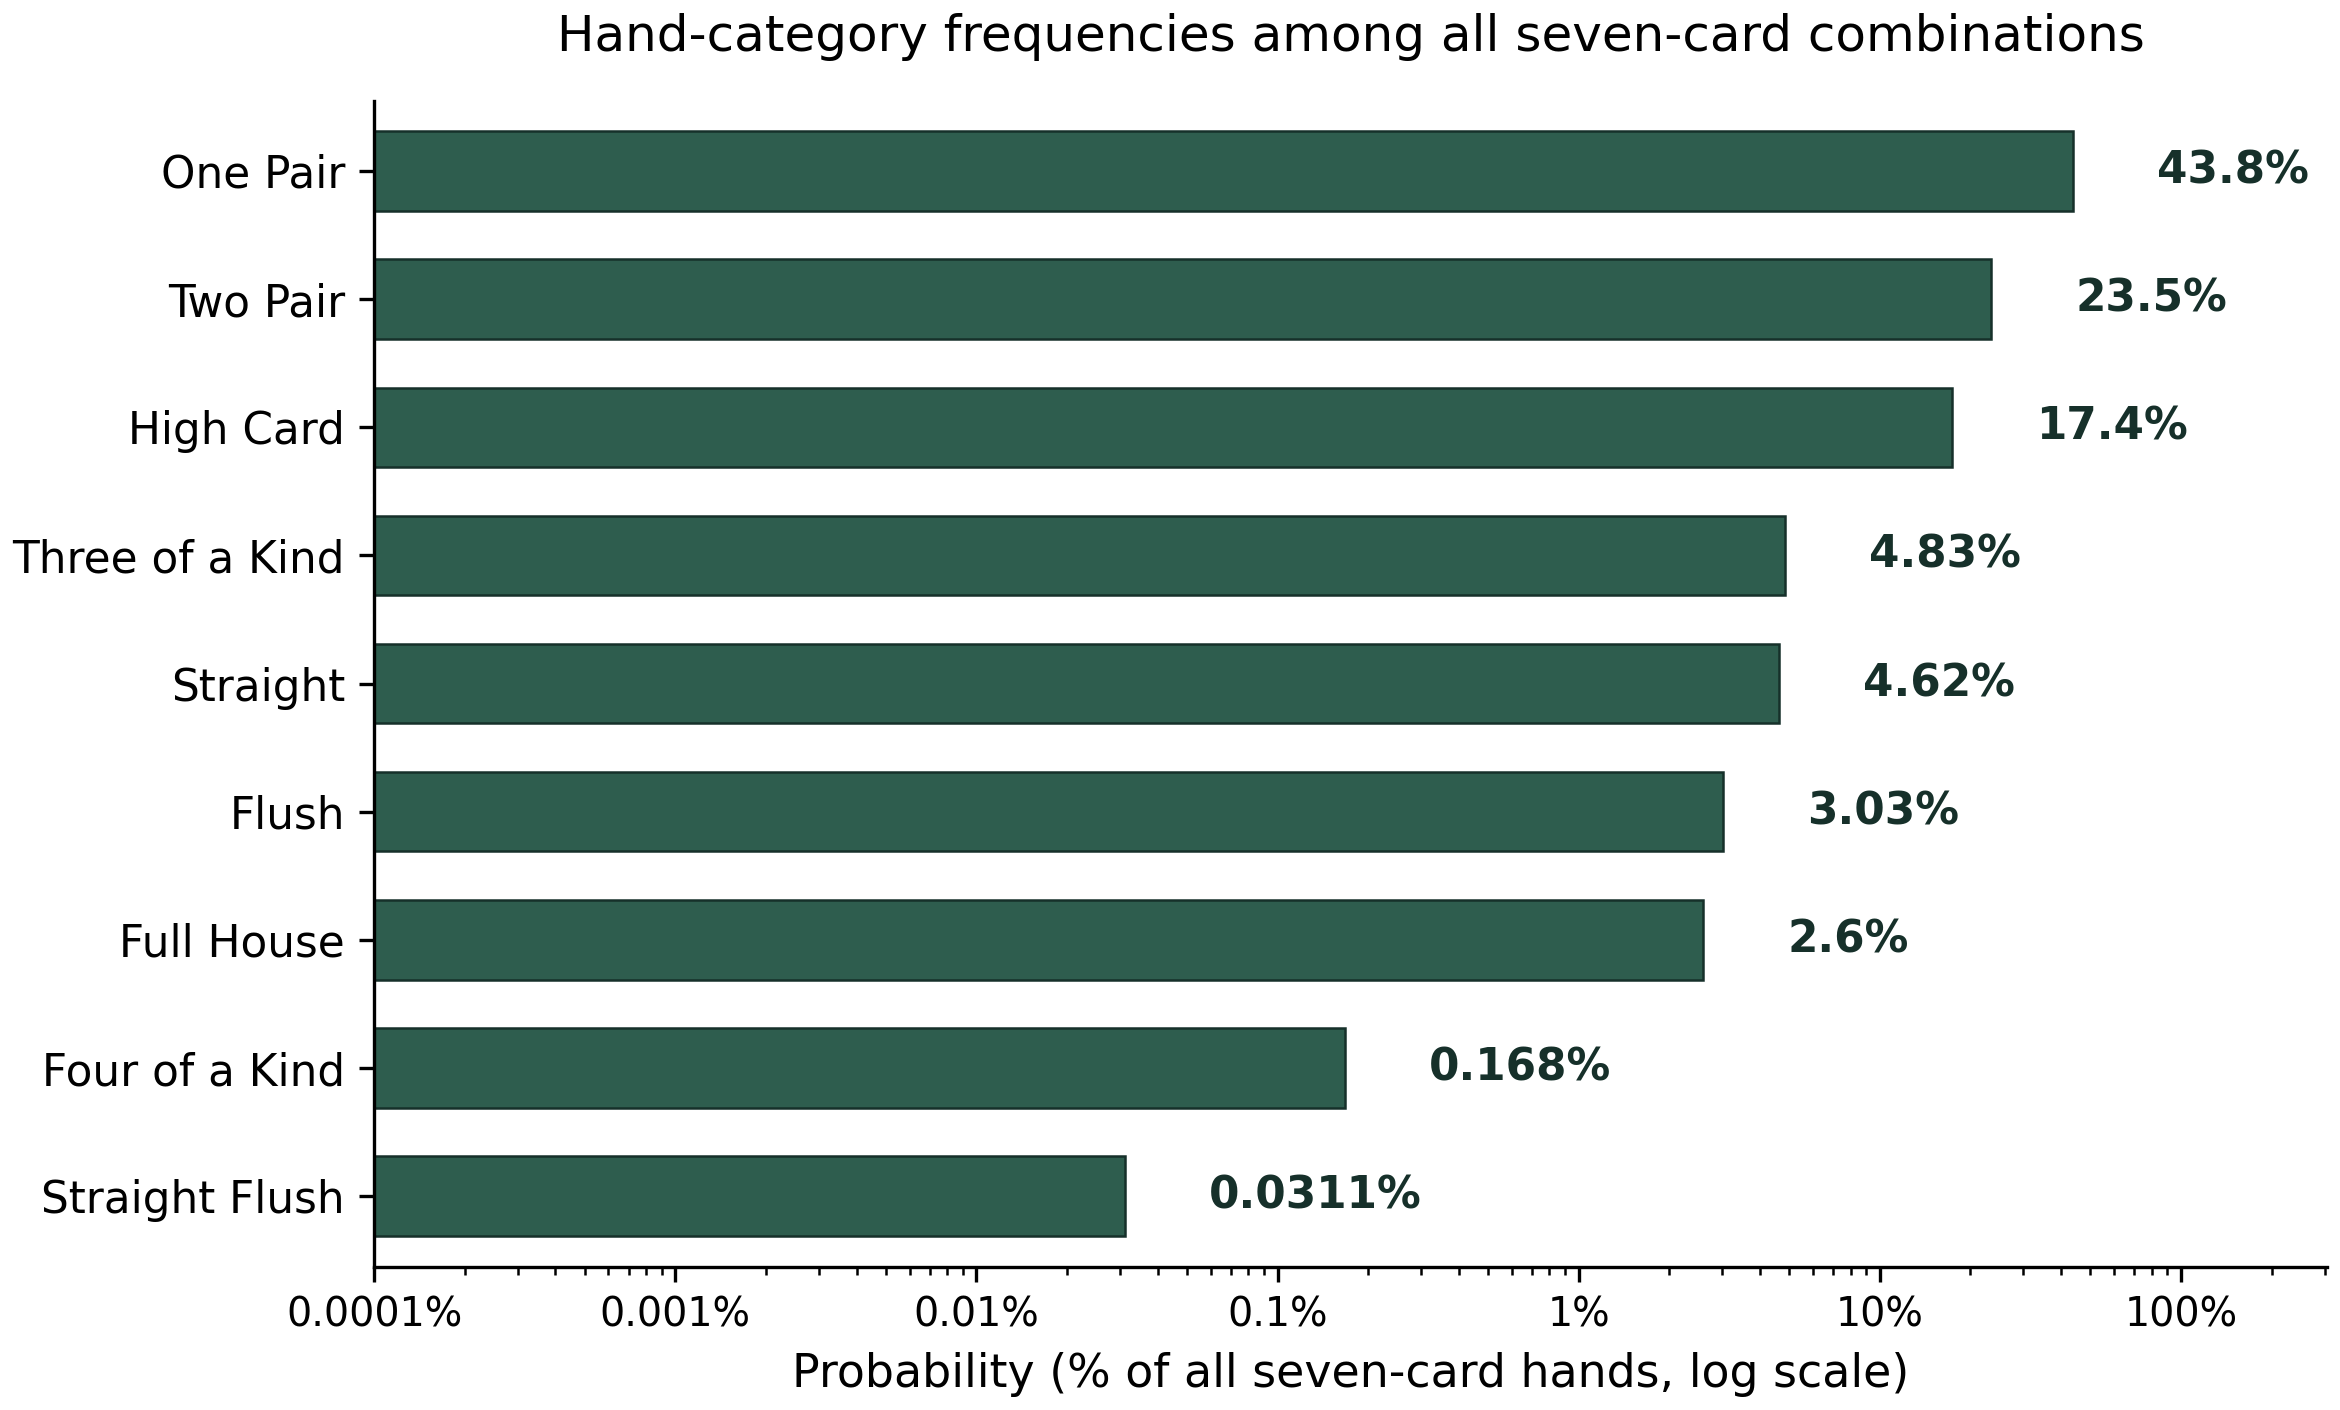
\includegraphics[width=0.92\textwidth]{figures/hand_ranks.png}
\caption{Frequency of each hand category among all $\binom{52}{7}$ seven-card combinations, on a logarithmic probability scale (categories ordered by seven-card frequency). Labels give percentages; the corresponding exact counts appear in Table~\ref{tab:ranks}.}
\label{fig:handranks}
\end{figure}

\subsection{Preflop equity}\label{sec:preflopequity}

The single most useful summary of a starting hand is its \emph{equity}: the probability of winning (with ties counted fractionally) if all remaining cards were dealt and all hands revealed. Equity against a single uniformly random opponent can be computed exactly by enumeration or estimated by simulation; Figure~\ref{fig:preflop} shows the values for all $169$ canonical hands. The structure is instructive. Pocket aces hold about $85\%$ equity; the worst hand, $7\clubsuit 2\diamondsuit$, holds about $35\%$---still far from hopeless heads-up, because even trash occasionally pairs or makes a backdoor straight. Suitedness is worth roughly $2$--$3$ equity points for high-card hands (flush potential), and connectedness adds a fraction of a point (straight potential). The same grid, computed against multiple simultaneous random opponents, compresses dramatically: against five random hands, AA retains roughly $49\%$ equity while $72$o falls under $5\%$, which is why multiway pots systematically reward speculative hands and punish dominated high-card holdings.

\begin{figure}[htbp]
\centering
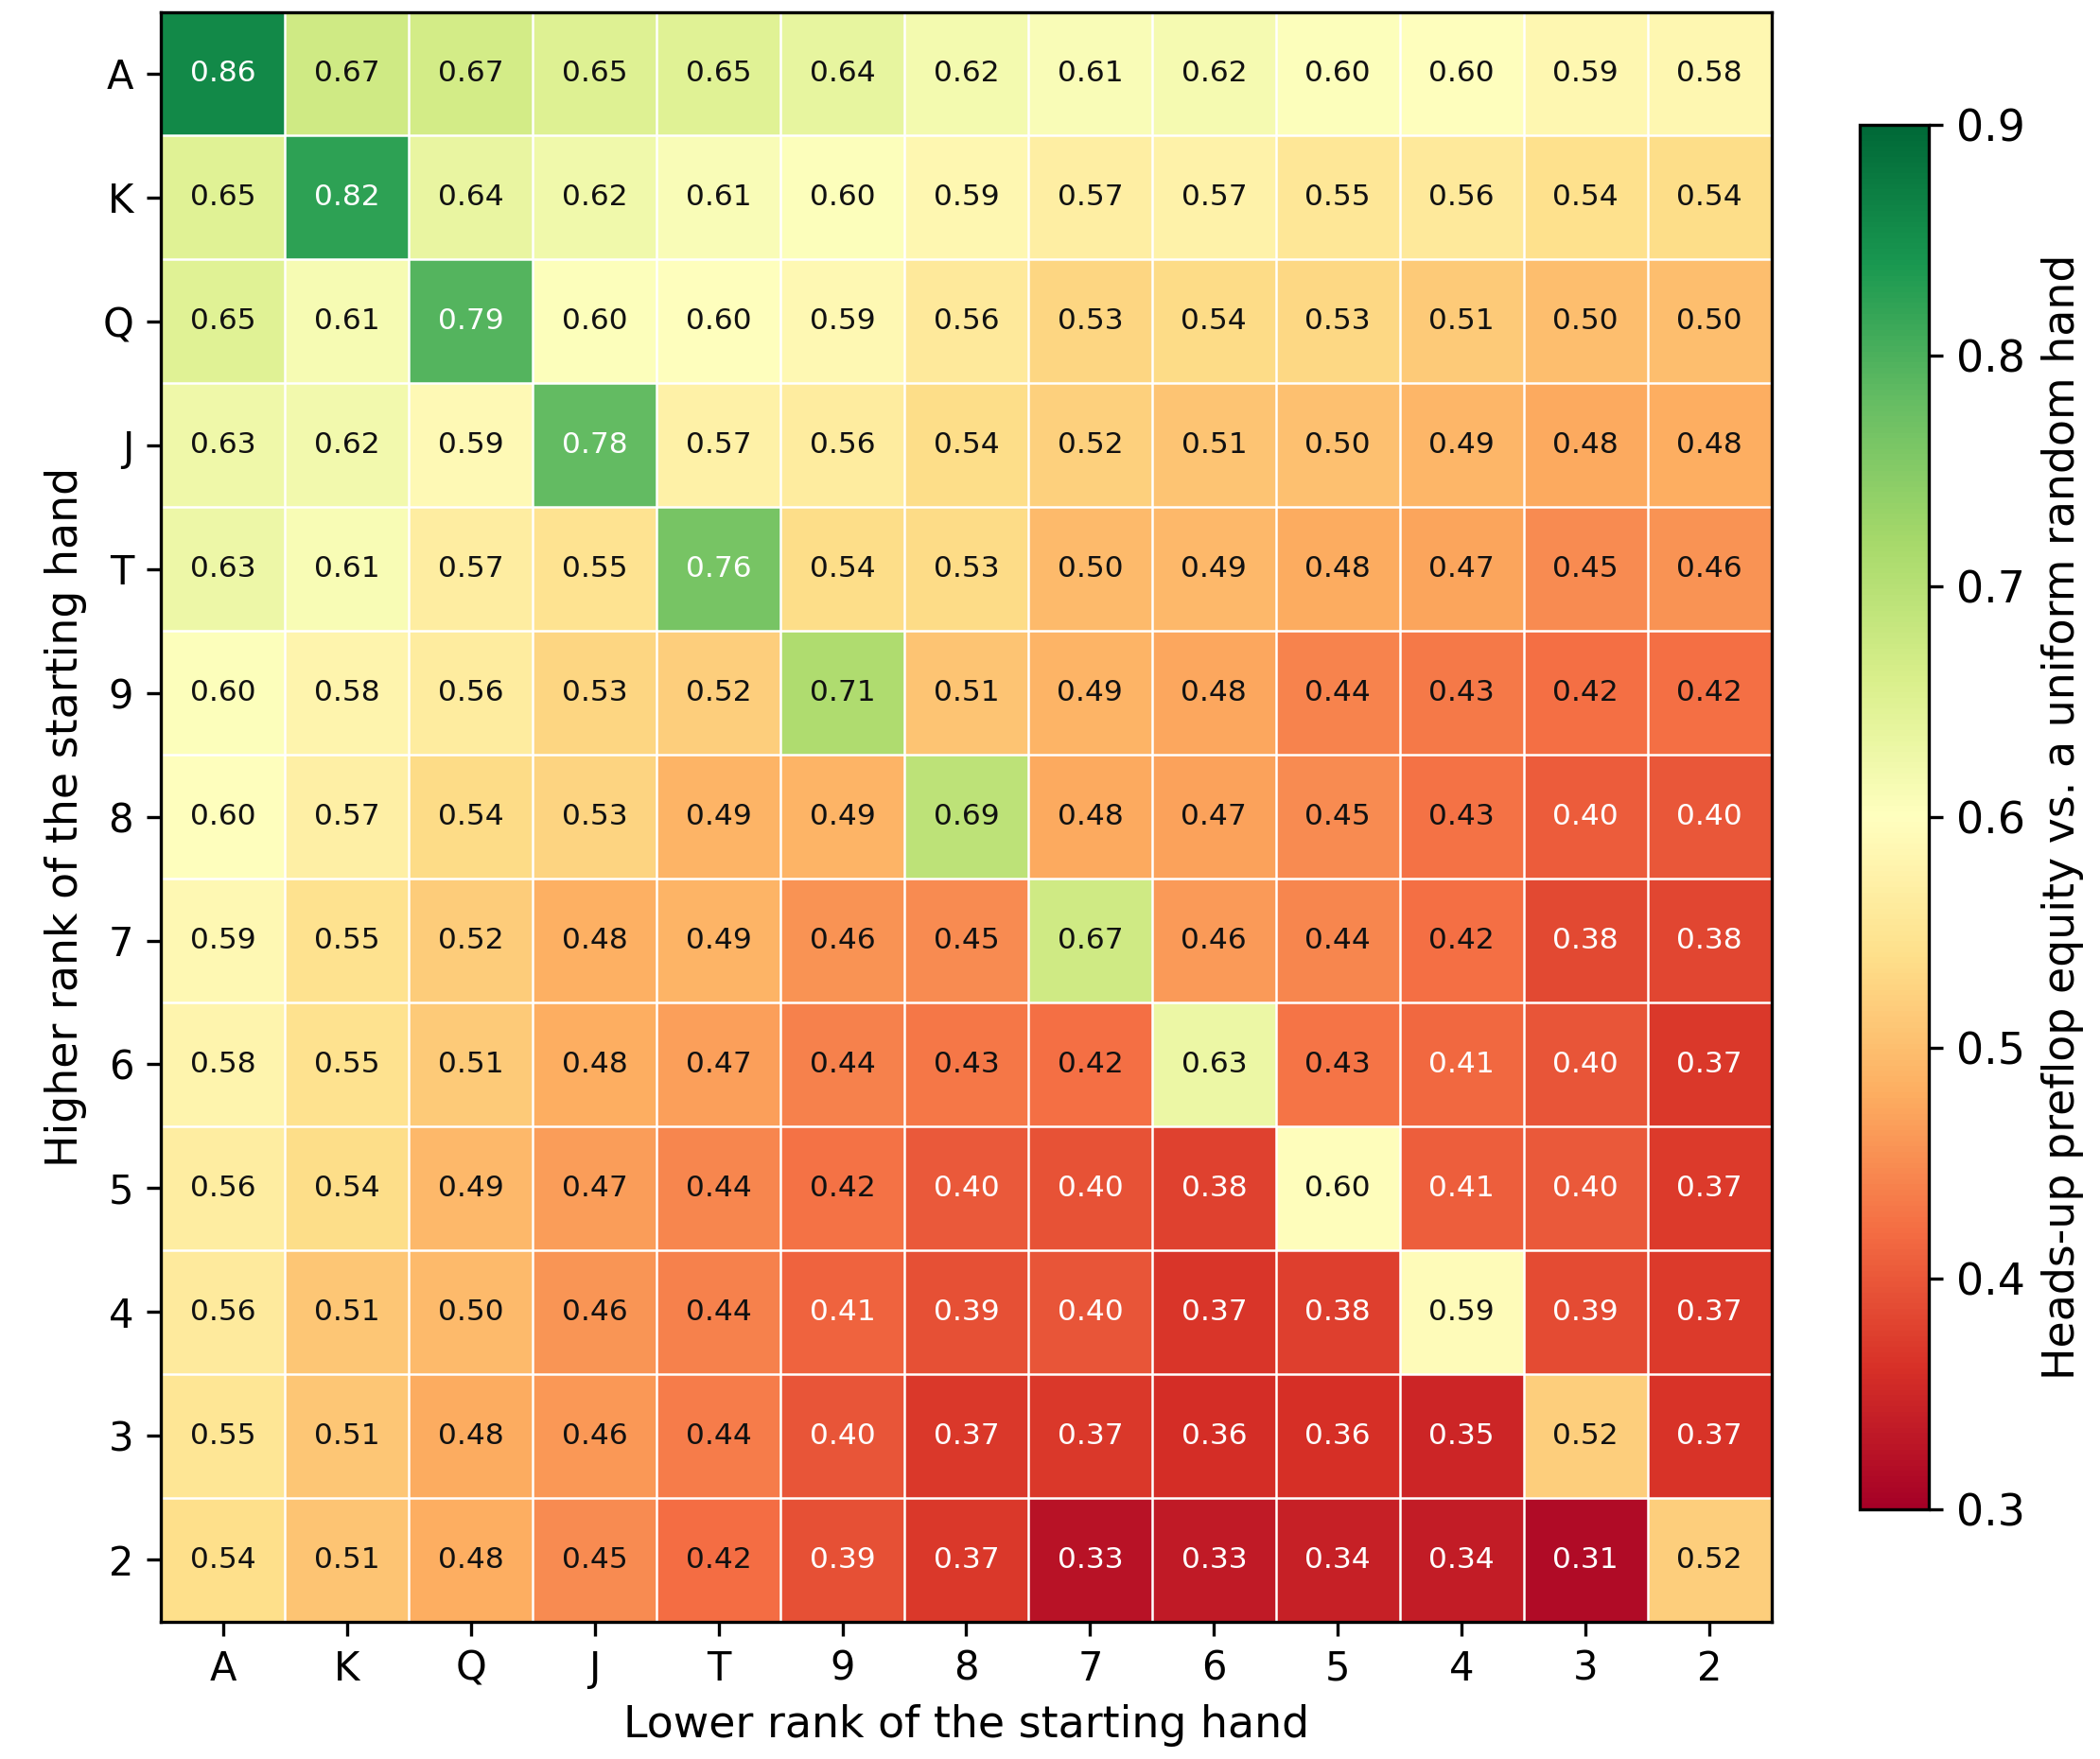
\includegraphics[width=0.86\textwidth]{figures/preflop_equity.png}
\caption{Heads-up preflop equity of all $169$ canonical starting hands against a uniformly random opponent, estimated by Monte Carlo simulation with $4{,}000$ runouts per hand. Values above the diagonal are suited hands; those below are offsuit.}
\label{fig:preflop}
\end{figure}

\subsection{Conditional probability and reads}

Once the flop arrives, hand strength must be conditioned on the visible cards. If a player holds a flush draw---four cards of one suit---then among the $47$ unseen cards, $9$ complete the flush, so by a direct application of the definition of conditional probability,
\begin{equation}\label{eq:flushdraw}
\Pr(\text{flush by river} \mid \text{flop}) = 1 - \frac{\binom{47}{2} - \binom{9}{1}\binom{38}{1} - \binom{9}{2}}{\binom{47}{2}} = 1 - \frac{\binom{38}{2}}{\binom{47}{2}} \approx 0.3497 .
\end{equation}
Poker players memorise the practical rule that follows from \eqref{eq:flushdraw}: with two cards to come, multiply the number of \emph{outs} by $4$; with one card to come, by $2$. The rule is accurate to within a couple of percentage points for the relevant range $1 \le \text{outs} \le 21$ precisely because it is the first-order binomial approximation of \eqref{eq:flushdraw}.

Bayes' theorem is the formal home of \emph{reading} an opponent. Write $H$ for a hypothesis about the opponent's holding (for instance, ``at least one club'') and $E$ for observed evidence (for instance, ``the opponent called a large bet on a two-club board''). Then
\begin{equation}\label{eq:bayes}
\Pr(H \mid E) = \frac{\Pr(E \mid H)\,\Pr(H)}{\Pr(E)},
\qquad
\Pr(E) = \sum_{H'} \Pr(E \mid H')\,\Pr(H') .
\end{equation}
Strong play requires an a priori model $\Pr(H)$ of the opponent's distribution (a \emph{range}) over holdings, and a behavioural likelihood $\Pr(E \mid H)$ describing how the opponent bets with each holding. Expert ``table reading'' is exactly the disciplined application of \eqref{eq:bayes}, updating the range after every action; opponent-modelling systems such as those reviewed by Billings et al.~\cite{billings2002challenge} mechanise the same computation.

\subsection{Pot odds, equity, and expected value}

Suppose the pot currently contains $P$ chips and a player faces a bet of $b$ chips. Calling costs $b$ to contest a pot of $P + b$, so the call is profitable in expectation against the bettor's distribution whenever the caller's equity $\eq$ satisfies
\begin{equation}\label{eq:potodds}
\eq \;>\; \frac{b}{P + b} .
\end{equation}
The right-hand side is called the \emph{pot odds} expressed as a required equity fraction. The inequality follows from a one-line expected-value computation: letting $W$ be the indicator of winning the pot outright (ignoring ties),
\begin{equation}\label{eq:evcall}
\E[\text{profit}] = \eq\,P - (1-\eq)\,b = \eq (P + b) - b ,
\end{equation}
which is positive exactly when \eqref{eq:potodds} holds. As a concrete example: facing a half-pot bet of $b = P/2$, the threshold is $P/2 \div 3P/2 = 1/3$; a player with a nine-out flush draw on the turn ($9/46 \approx 0.196$ from \eqref{eq:flushdraw} with one card to come) does not have direct odds and must either fold or justify the call through \emph{implied odds}---expected additional winnings $I$ on later streets when the draw completes, replacing \eqref{eq:potodds} by
\begin{equation}
\eq \;>\; \frac{b}{P + b + I} .
\end{equation}

Expected value is the fundamental quantity of the entire subject. If a strategy profile induces a distribution $p$ over terminal outcomes with payoffs $v(z)$, the value of the strategy is
\begin{equation}\label{eq:evdef}
v = \E_p[v] = \sum_z p(z)\, v(z),
\qquad \Var[v] = \sum_z p(z)\,(v(z) - v)^2 .
\end{equation}
Maximising \eqref{eq:evdef} is the correct objective only when the distribution $p$ is known or estimated; much of Sections~\ref{sec:gametheory}--\ref{sec:rl} is devoted to the harder case where $p$ is shaped by strategic opponents who hide information.

\subsection{Variance, swings, and the Kelly criterion}

Poker outcomes are dominated by variance. In a typical no-limit game, the per-hand profit of a solid player has standard deviation on the order of $10$--$15$ big blinds (bb) while the expected profit is a few tenths of a bb; the ratio of noise to signal is therefore $20$--$50$ per hand. It follows from the central limit theorem that after $n$ hands the cumulative profit is approximately normal with mean $n\mu$ and standard deviation $\sqrt{n}\,\sigma$, so the number of hands needed to be $95\%$ confident of a positive cumulative result is
\begin{equation}\label{eq:handsneeded}
n \;\ge\; \left( \frac{1.645\,\sigma}{\mu} \right)^{2} .
\end{equation}
With $\sigma = 12$\,bb and $\mu = 0.3$\,bb this is roughly $43{,}000$ hands---a first quantitative explanation of why judging poker skill from a single session is statistically meaningless, and why the simulation study of Section~\ref{sec:experiments} requires tens of thousands of hands to separate its agents.

Bankroll management is the repeated-investment version of the same computation. If a player wins $b$ units per unit staked with probability $p > 1/2$, Kelly's classical result~\cite{kelly1956new} states that the fraction of the bankroll to risk that maximises the asymptotic growth rate is
\begin{equation}\label{eq:kelly}
f^{*} = \frac{b\,p - (1-p)}{b} = p - \frac{1-p}{b} ,
\end{equation}
obtained by maximising $\E[\log(1 + f X)]$ over the stake fraction $f$. Because the log objective penalises ruin superlinearly, the Kelly fraction is conservative relative to the naive $\mu/\sigma^{2}$ sizing; serious players typically adopt a fraction of Kelly between one quarter and one half to buffer estimation error in $p$ and $b$. The deeper lesson transfers directly to the algorithms of Section~\ref{sec:rl}: any learning or search procedure whose per-decision stakes are sized by noisy estimates must temper its aggression in proportion to estimation uncertainty.

% !TeX root = ../main.tex
\section{Hand Evaluation, Monte Carlo, and Expert Systems}\label{sec:evaluation}

Before any strategic reasoning can occur, a program must answer two primitive questions quickly and exactly: \emph{which five-card hand does a player hold} (ranking), and \emph{how strong is a holding against a specified field of opponents} (equity). This section develops both primitives and then assembles them into the first rung of the algorithmic ladder: a rule-based expert system and a Monte Carlo simulation agent, the two paradigms that dominated computer poker before game-theoretic methods arrived.

\subsection{Exact hand evaluation}

A Hold'em evaluator is a function from seven cards to a totally ordered score. The natural construction exploits the fact that a player's effective hand is the \emph{best} of the $\binom{7}{5}=21$ five-card subsets:
\begin{equation}\label{eq:eval}
\operatorname{score}(c_1,\dots,c_7) \;=\; \max_{S \in \binom{[7]}{5}} \operatorname{rank}_5(S),
\end{equation}
where $\operatorname{rank}_5$ maps a five-card hand to a lexicographic tuple (category, primary kickers, \dots, final kicker). Because the nine categories of Section~\ref{sec:rankings} are mutually exclusive at fixed card multiplicity, and within-category comparison reduces to comparing kickers in order, $\operatorname{rank}_5$ takes values in a set of $7{,}462$ distinct equivalence classes, which pack into a single machine integer. Our implementation encodes $(\text{category}, k_1, k_2, \dots)$ as base-15 digits, so that \eqref{eq:eval} becomes 21 integer maximisations---about $1.5$\,ns per evaluation on commodity hardware. Production evaluators go further: the widely used two-plus-two table-driven evaluator precomputes multi-card lookup tables over the card space and evaluates seven cards in seven $O(1)$ table probes. The exact method matters little for correctness---all sound evaluators induce the same total order---but matters greatly for the training loops of Sections~\ref{sec:cfr} and~\ref{sec:rl}, whose wall-clock budgets are consumed almost entirely by evaluation.

\subsection{Monte Carlo equity estimation}\label{sec:mc}

Exact ranking solves showdowns, but decisions require \emph{equity}: the win probability of a holding against a distribution of opponent holdings and future boards. For a single uniformly random opponent this expectation has a closed form only in trivial cases; the standard tool is Monte Carlo estimation. Fix the player's hole cards $h$ and the visible board $B$, let $U$ denote the unseen cards, and let $e$ be the true equity. A \emph{runout} samples the opponent's hole cards $o \sim U$ and the board completion $r \sim U \setminus \{o\}$ uniformly without replacement; the estimator draws $n$ i.i.d.\ runouts and returns
\begin{equation}\label{eq:mcest}
\begin{split}
\hat e_n \;=\; \frac{1}{n}\sum_{i=1}^{n} W_i, \qquad
W_i \;=\;{}& \mathbf{1}\{\operatorname{score}(h \cup r_i) > \operatorname{score}(o_i \cup r_i)\} \\
&+ \tfrac{1}{m_i + 1}\,\mathbf{1}\{\text{tie against $m_i$ opponents}\},
\end{split}
\end{equation}
where $o_i$ is the sampled opponent holding, $r_i$ the sampled board completion, and a tie splits the pot among the $m_i + 1$ tied hands.

\begin{proposition}\label{prop:mc}
$\hat e_n$ is an unbiased estimator of $e$ with $\Var(\hat e_n) \le e(1-e)/n$, with equality when no ties occur. Consequently $\SE(\hat e_n) \le \sqrt{e(1-e)/n} \le \tfrac{1}{2\sqrt n}$, and by the de Moivre--Laplace central limit theorem an asymptotic $95\%$ confidence interval is $\hat e_n \pm 1.96\,\sqrt{\hat e_n(1-\hat e_n)/n}$.
\end{proposition}
\begin{proof}
Each $W_i$ is an independent draw of the random variable $W = \mathbf{1}\{\text{win}\} + \text{(fractional tie)}$, whose mean is $e$ by construction of the uniform sampling measure; ties contribute fractional mass so that $\E[W]$ equals the exact split-pot equity. Since $W \in [0,1]$ with $\E[W] = e$, the Bhatia--Davis bound gives $\Var(W) \le e(1-e)$, with equality exactly when $W$ is $\{0,1\}$-valued (no fractional ties); hence $\Var(\hat e_n) \le e(1-e)/n$, maximised at $e = 1/2$.
\end{proof}

The $1/\sqrt{n}$ decay is the governing constraint on every sampling-based poker agent: doubling precision quadruples the simulation budget. Figure~\ref{fig:mcprecision} plots the standard error \eqref{prop:mc} against $n$ and marks the two budgets used by our implementation: $n = 300$ for batch (tournament) play, giving $\SE \approx 2.9$ equity points, and $n = 1500$ for interactive play with a 220\,ms time budget, giving $\SE \approx 1.3$ points. The practical reading is sobering: even $1{,}500$ runouts cannot distinguish a $52\%$ equity from a $49\%$ equity at $95\%$ confidence, yet such margins decide most real bets. Variance-reduction techniques (antithetic pairing of high/low runouts, stratified sampling of opponent hands by canonical class) can shave constant factors, but the square-root wall is information-theoretic: an agent that wants sharper beliefs must either enumerate (exactly, at combinatorial cost) or \emph{condition on fewer unknowns}---which is precisely what the abstraction machinery of Section~\ref{sec:cfr} achieves by design.

\begin{figure}[htbp]
\centering
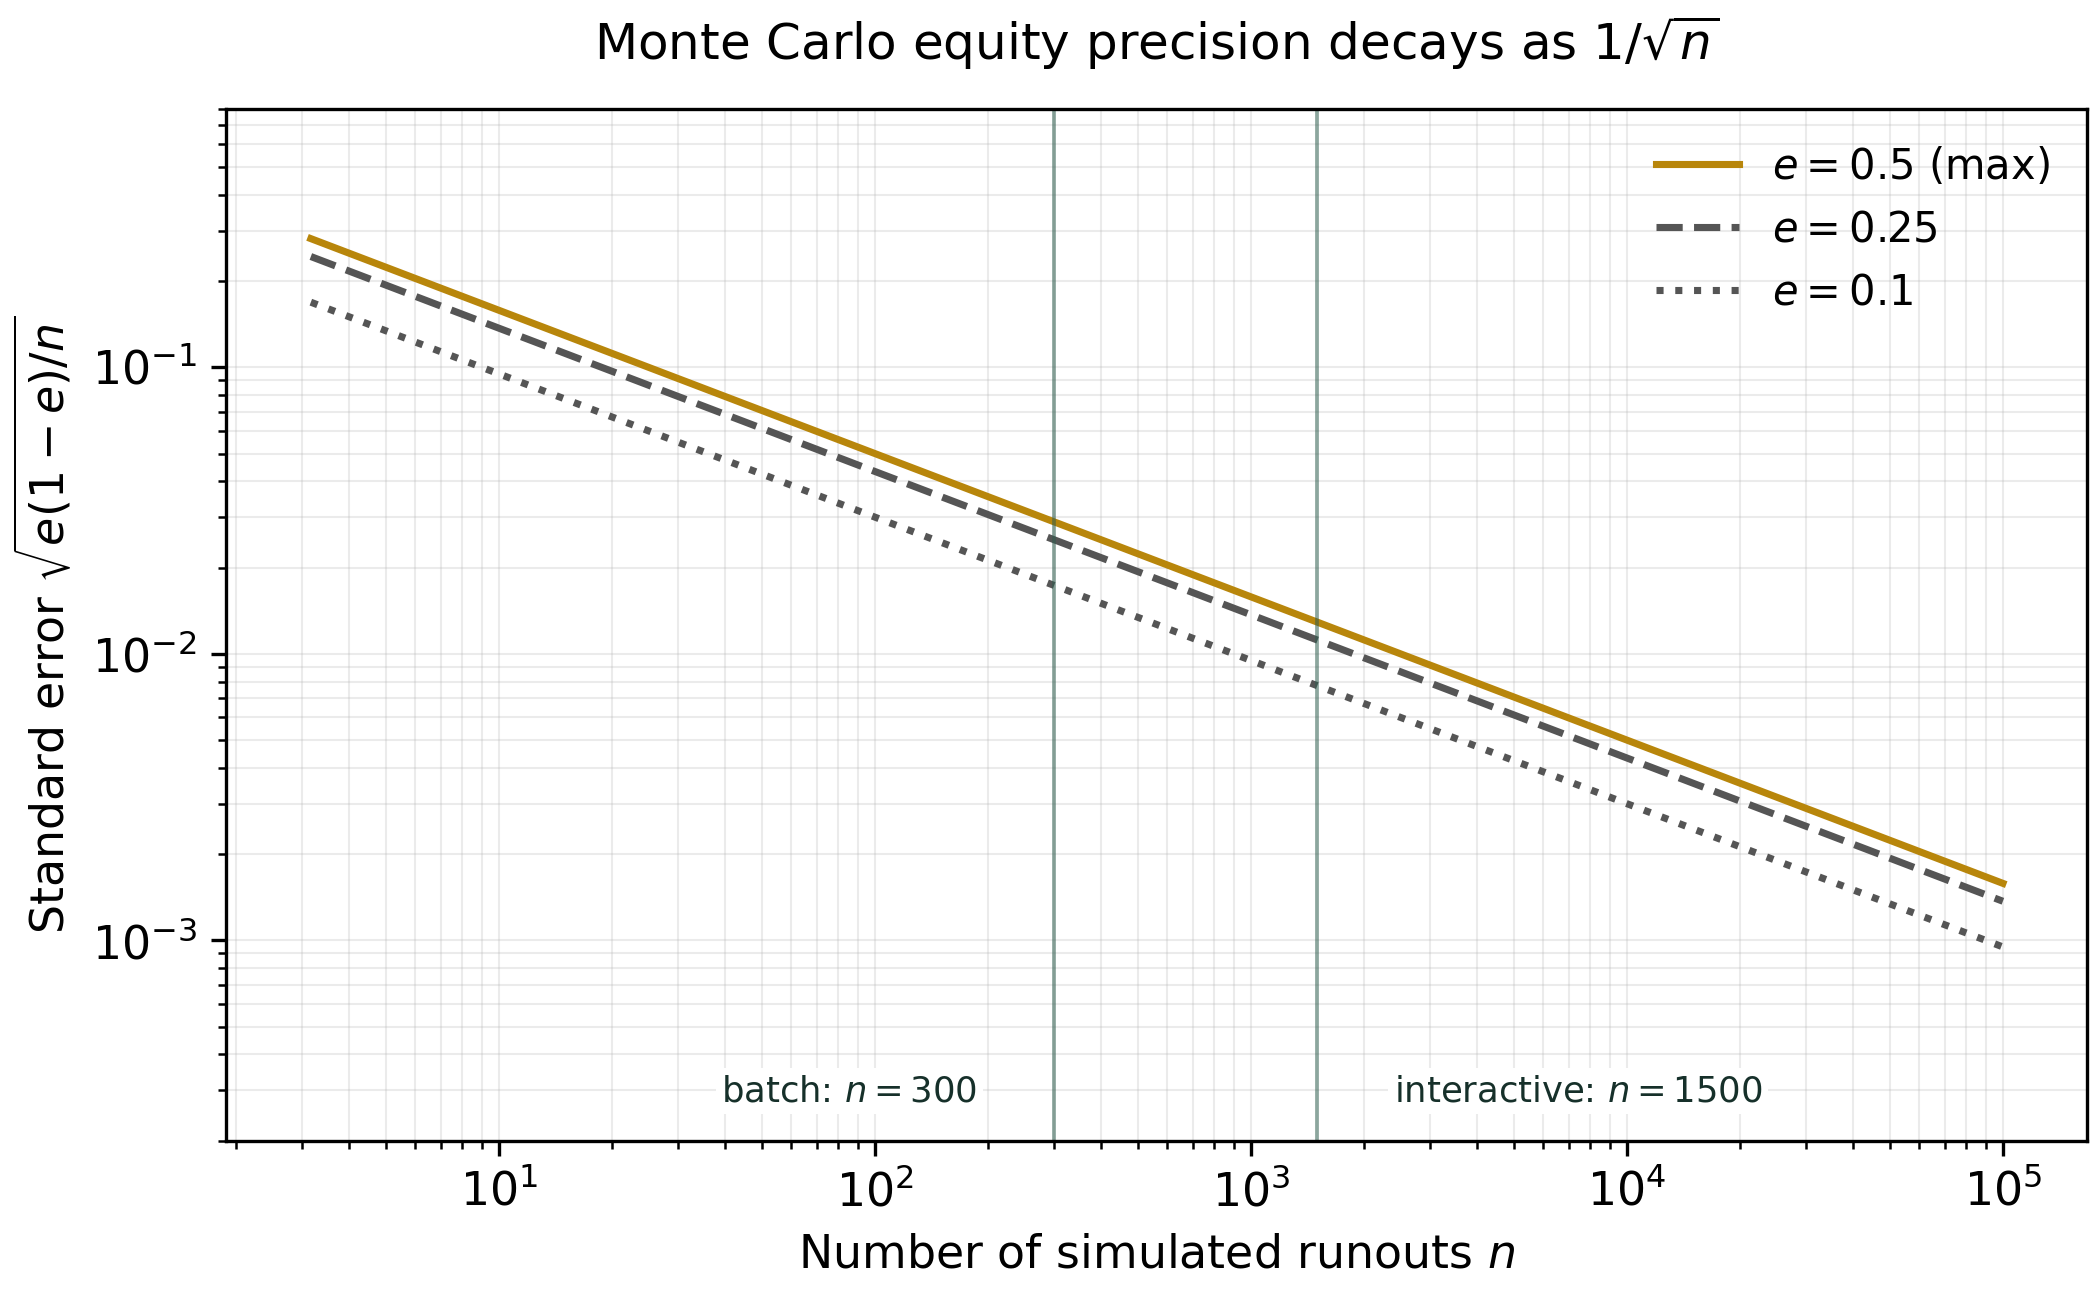
\includegraphics[width=0.82\textwidth]{figures/mc_precision.png}
\caption{Standard error of the Monte Carlo equity estimator \eqref{eq:mcest} as a function of the number of simulated runouts, for true equities $e \in \{0.5, 0.25, 0.1\}$ (the no-tie worst case). The vertical lines mark the two simulation budgets of our Monte Carlo agent: the batch budget $n = 300$ (worst-case $\SE \approx 2.9$ percentage points) and the interactive budget $n = 1500$ ($\SE \approx 1.3$ points).}
\label{fig:mcprecision}
\end{figure}

\subsection{Rule-based expert systems}

The oldest and still most common commercial paradigm encodes human expert knowledge as a decision procedure over computed statistics. Our implementation, which we call the \emph{rule agent}, is a faithful miniature of this school. At each decision point it computes three quantities: a \emph{strength} estimate $s \in [0,1)$---preflop, a table lookup of the 169 canonical hands' Monte Carlo equities (Figure~\ref{fig:preflop}); postflop, a made-hand percentile with additive draw bonuses---a \emph{position class} from $\{\text{EP}, \text{MP}, \text{LP}, \text{SB}, \text{BB}\}$, and the \emph{pot-odds threshold} $b/(P+b)$ of \eqref{eq:potodds}. Decision rules then combine them: open-raise when $s$ clears a position-dependent threshold (tighter in early position, looser on the button), three-bet premium holdings, call when $s$ exceeds the required equity plus a multiway safety margin $0.03 + 0.025\,\min(3, \text{opponents})$, value-bet strong made hands, and bluff at a low fixed frequency when last to act. Algorithm~\ref{alg:rule} gives the complete decision procedure.

\begin{algorithm}[htbp]
\DontPrintSemicolon
\caption{Rule-based decision at one betting node (our \emph{rule agent}; rules are priority-ordered, first match fires).}\label{alg:rule}
\KwIn{state (hole, board, pot $P$, to-call $b$, position $\rho$, opponents $m$), random draw $r \sim U(0,1)$}
\KwOut{action $\in$ \{fold, check/call, raise $\tfrac12$-pot, raise pot\}}
$s \leftarrow$ preflop-equity lookup or made-hand percentile $+$ draw bonuses\;
\If{$b = 0$}{
  \uIf{preflop \textbf{and} $s \ge \theta_{\text{open}}(\rho)$}{
    \eIf{$s \ge 0.62$ \textbf{and} $r < 0.35$}{emit pot-sized raise}{emit half-pot raise}\;
  }
  \uElseIf{postflop \textbf{and} $s \ge 0.84$}{
    \eIf{$r < 0.4$}{emit pot-sized raise}{emit half-pot raise}\;
  }
  \uElseIf{postflop \textbf{and} $s \ge 0.72$}{emit half-pot raise (value bet)\;}
  \uElseIf{postflop \textbf{and} $s \ge 0.56$ \textbf{and} $r < 0.45$}{emit half-pot raise (probe)\;}
  \uElseIf{postflop \textbf{and} $\rho = \mathrm{LP}$ \textbf{and} $s < 0.45$ \textbf{and} $r < 0.16$}{emit half-pot raise (bluff)\;}
  \Else{check (fold-option hands check behind)\;}
}
\Else{
  $\theta \leftarrow b/(P+b) + 0.03 + 0.025\min(3,m) - \mathbb{1}[\rho \in \{\text{SB},\text{BB}\}]\cdot 0.02$\;
  \If{preflop \textbf{and} $s \ge 0.68$ \textbf{and} raises this street $< 3$ \textbf{and} $r < 0.55$}{emit 3-bet\;}
  \If{postflop \textbf{and} $s \ge 0.80$ \textbf{and} raises this street $< 2$ \textbf{and} $r < 0.4$}{emit raise\;}
  \If{$s \ge \theta$}{call\;}
  \If{$b/(P+b) < 0.15$ \textbf{and} $s \ge 0.42$}{call (cheap peeling / set-mining)\;}
  \If{$b/(P+b) < 0.22$ \textbf{and} $s \ge b/(P+b) - 0.04$ \textbf{and} $r < 0.5$}{call (implied odds)\;}
  \Return fold\;
}
\end{algorithm}

The strengths of this paradigm are transparency (every action is explainable in terms a human recognises---the agent's user interface displays exactly these threshold comparisons), speed (microseconds per decision), and robustness against catastrophic error. Its weaknesses are equally structural. First, the thresholds are \emph{static}: the agent cannot adapt to an opponent who folds too much or calls too much, whereas a best responder profits precisely from such regularities. Second, and more fundamentally, the rule agent has no theory of \emph{balanced ranges}: because its aggression depends only on its own card strength, its betting ranges are transparently polarised or merged, and its bluff frequency is an arbitrary constant rather than a quantity chosen to make the opponent indifferent. A game-theoretic opponent can therefore exploit it systematically, a defect that Section~\ref{sec:experiments} quantifies in win-rate terms. The Monte Carlo agent improves the \emph{estimation} half of the problem---it replaces the heuristic strength $s$ with a live simulation against the actual number of opponents, with an honest confidence interval---but inherits the same static decision thresholds, so its fate against adaptive opponents is similar.

Both paradigms share a deeper limitation: they treat each decision in isolation, as a myopic expected-value calculation against a \emph{fixed} model of the opponents. Poker's central difficulty is that the model is not fixed---opponents' strategies respond to ours, and their private cards generate adversarial uncertainty that no amount of sampling removes. Formalising this observation requires the language of game theory, to which we now turn.

% !TeX root = ../main.tex
\section{Game-Theoretic Foundations}\label{sec:gametheory}

\subsection{Extensive-form games with imperfect information}\label{sec:efg}

The correct formal model for poker is a finite extensive-form game with imperfect information. It consists of:
\begin{enumerate}[leftmargin=1.6em,itemsep=1pt]
\item a finite game tree rooted at $h_0$; internal nodes $h$ belong to a player-mapping $P: H \to N \cup \{c\}$, where $N = \{1, \dots, n\}$ are the players and $c$ is the chance player;
\item chance nodes prescribe probability $\sigma_c(h, a)$ to each child $h \cdot a$ (in Hold'em, uniform over the unseen cards);
\item payoffs $u_i: Z \to \mathbb{R}$ at terminal nodes $z \in Z$ (in Hold'em, chip deltas);
\item for each player $i$, a partition $\mathcal{I}_i$ of that player's decision nodes into \emph{information sets} $I$: nodes in one $I$ are indistinguishable to $i$ because they differ only in information $i$ cannot observe (opponents' cards).
\end{enumerate}
A player's memory of its own past observations is encoded by the partition: the game has \emph{perfect recall} if, whenever two nodes $h, h'$ lie in the same information set of player $i$, the sequence of $i$'s information sets and actions leading to $h$ and to $h'$ is identical---informally, the player never forgets what it once knew or did. All poker variants have perfect recall, which matters because of Kuhn's theorem: with perfect recall, behavioural strategies (independent action distributions at each information set) are payoff-equivalent to mixed strategies (distributions over deterministic plans), and the two representations can be interchanged freely~\cite{kuhn1953extensive}. Every algorithm in this paper therefore operates on behavioural strategies $\sigma_i$, which assign to each $I \in \mathcal{I}_i$ a distribution over the actions legal at $I$.

The number of information sets is the true measure of a poker game's size. Heads-up limit Hold'em has about $10^{17}$ of them; heads-up no-limit, on the order of $10^{160}$ counting distinct bet sizes; six-player no-limit is larger still~\cite{sandholm2015abstraction}. Any tabular method that touches each information set once is hopeless at this scale---a fact that drives every abstraction decision in Section~\ref{sec:cfr}.

\subsection{Nash equilibrium and its guarantees}\label{sec:nash}

A strategy profile $\sigma = (\sigma_1, \dots, \sigma_n)$ is a \emph{Nash equilibrium} if no player gains by unilateral deviation: for every $i$ and every alternative $\sigma_i'$,
\begin{equation}\label{eq:nash}
u_i(\sigma_i', \sigma_{-i}) \;\le\; u_i(\sigma).
\end{equation}
Nash's theorem guarantees that every finite game has at least one such profile (in mixed strategies; with perfect recall, in behavioural strategies)~\cite{nash1950equilibrium}. The concept's computational meaning for two-player \emph{zero-sum} games is sharper. Define a player's \emph{best response} value $\br_i(\sigma_{-i}) = \max_{\sigma_i'} u_i(\sigma_i', \sigma_{-i})$ and the \emph{exploitability} of a profile by
\begin{equation}\label{eq:expl}
\varepsilon(\sigma) \;=\; \tfrac12\!\left[\br_1(\sigma_2) + \br_2(\sigma_1)\right] \;=\; \tfrac12\!\left[\max_{\sigma_1'} u_1(\sigma_1', \sigma_2) - \min_{\sigma_2'} u_1(\sigma_1, \sigma_2')\right],
\end{equation}
which vanishes exactly at equilibrium. Two consequences make equilibrium play the reference standard for competitive poker AI. First, by von Neumann's minimax theorem the zero-sum game has a \emph{value} $v^*$: any equilibrium profile attains it, player~1 can guarantee at least $v^*$ against \emph{any} opponent, and player~2 can hold any opponent to at most $v^*$. A maximally unexploitable strategy is therefore also a maximally safe one. Second, approximate equilibria inherit approximate safety: if $\varepsilon(\sigma) \le \epsilon$, then a best response against $\sigma$ earns at most $v^* + \epsilon$, \emph{regardless of the exploiter's knowledge or adaptivity}. This is the formal licence to search for $\epsilon$-equilibria of abstracted games and treat the result as robust---the licence under which Cepheus, Libratus, and Pluribus were built~\cite{bowling2015ceph,brown2017libratus,brown2019pluribus}.

Beyond two players these guarantees dissolve. With three or more players the game is no longer zero-sum (one player's loss is not another's gain), equilibrium values are not interchangeable, and some equilibria are collusively bad for individual players: in a six-player game, a strategy that is a best response to one profile of opponents can lose heavily against a different profile of the \emph{same strength}. Equilibrium strategy in multiplayer poker is therefore a \emph{robustness heuristic}---a guarantee against being the table's designated victim---rather than an optimality certificate. This is exactly how Pluribus was evaluated and is why the six-agent study of Section~\ref{sec:experiments} reports pairwise-style aggregate statistics rather than exploitability~\cite{brown2019pluribus}.

\subsection{Why perfect-information methods fail}

Backward induction on a game tree requires evaluating nodes; a node's value is well-defined only when the evaluator can condition on everything the mover knows. In poker the mover's knowledge is coarser than the tree: two nodes in one information set demand one action distribution yet differ in continuation values, because the hidden cards alter every downstream payoff. Any procedure that solves subtrees independently---alpha--beta search, expectimax, dynamic programming over the tree---silently conditions on the hidden state and thereby assumes the mover can read opponents' cards. The result is a strategy whose apparent value is an unreachable upper bound, and whose realised value against a live opponent collapses: a ``best strategy against known cards'' bluffs never and folds to every raise.

The failure has a constructive side: the correct equilibrium behaviour in imperfect-information games is generally \emph{mixed}. The trivial game rock--paper--scissors (a one-move simultaneous game) makes the point irreducibly: any deterministic strategy is exploited with certainty, and the unique equilibrium randomises uniformly over the three actions. Poker differs only in that the mixing probabilities are non-obvious, card-dependent, and coupled across a vast tree. The next example shows that even in the smallest poker game the mixing probabilities obey exact arithmetic that no intuition produces unaided.

\subsection{A complete worked example: Kuhn poker}\label{sec:kuhn}

Kuhn poker is the smallest game recognisably belonging to the poker family~\cite{kuhn1953extensive}. The deck has three cards $J < Q < K$; each player antes one unit and receives one card; bet size is fixed at one unit. Player~1 (P1) acts first and may check or bet; if P1 bets, P2 calls or folds; if P1 checks, P2 checks (showdown) or bets, whereupon P1 calls or folds. The game has 12 information sets---six per player (one per card at the first decision, one per card at the second)---and can be solved exactly.

\begin{figure}[htbp]
\centering
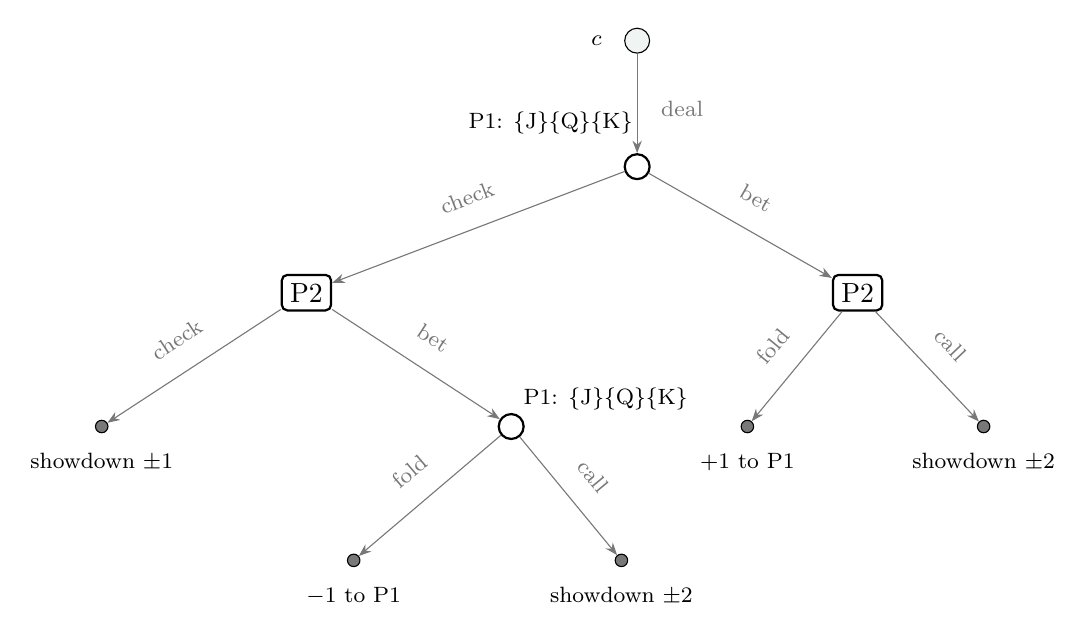
\begin{tikzpicture}[
  chn/.style={circle, draw, fill=boxbg, inner sep=1.5pt, minimum size=9pt},
  p1n/.style={circle, draw, thick, inner sep=1.5pt, minimum size=9pt},
  p2n/.style={rectangle, draw, thick, rounded corners=2pt, inner sep=3pt},
  term/.style={circle, draw, fill=rulegray, inner sep=0pt, minimum size=4.5pt},
  lab/.style={font=\footnotesize, midway, sloped, above=8pt, inner sep=0.5pt},
  nlab/.style={font=\footnotesize, inner sep=1pt},
  arr/.style={-{Stealth[length=4.5pt]}, rulegray}
]
  % ---------------- nodes (generously spaced coordinates) ----------------
  \node[chn] (root) at (0,0) {};
  \node[nlab, left=7pt of root] {$c$};
  \node[p1n] (p1) at (0,-1.6) {};
  \node[p2n] (p2k) at (-4.2,-3.2) {P2};
  \node[p2n] (p2b) at (2.8,-3.2) {P2};
  \node[p1n] (p1c) at (-1.6,-4.9) {};
  \node[term] (t1) at (-6.8,-4.9) {};
  \node[term] (t4) at (1.4,-4.9) {};
  \node[term] (t5) at (4.4,-4.9) {};
  \node[term] (t2) at (-3.6,-6.6) {};
  \node[term] (t3) at (-0.2,-6.6) {};
  % information-set labels, each placed in a verified clear zone
  \node[nlab] at (-1.1,-1.05) {P1: \{J\}\{Q\}\{K\}};
  \node[nlab] at (-0.4,-4.55) {P1: \{J\}\{Q\}\{K\}};
  % payoff labels, attached below their terminal dots
  \node[nlab, below=6pt of t1] {showdown $\pm 1$};
  \node[nlab, below=6pt of t2] {$-1$ to P1};
  \node[nlab, below=6pt of t3] {showdown $\pm 2$};
  \node[nlab, below=6pt of t4] {$+1$ to P1};
  \node[nlab, below=6pt of t5] {showdown $\pm 2$};
  % ---------------- edges ----------------
  \draw[arr] (root) -- node[font=\footnotesize, inner sep=0.5pt, right=8pt, pos=0.55] {deal} (p1);
  \draw[arr] (p1) -- node[lab] {check} (p2k);
  \draw[arr] (p1) -- node[lab] {bet} (p2b);
  \draw[arr] (p2k) -- node[lab] {check} (t1);
  \draw[arr] (p2k) -- node[lab] {bet} (p1c);
  \draw[arr] (p1c) -- node[lab] {fold} (t2);
  \draw[arr] (p1c) -- node[lab] {call} (t3);
  \draw[arr] (p2b) -- node[lab] {fold} (t4);
  \draw[arr] (p2b) -- node[lab] {call} (t5);
\end{tikzpicture}
\caption{The Kuhn poker tree (card-deal branches and per-card information sets suppressed; each decision node shown aggregates three information sets, one per private card). Both players see only their own card, so every decision aggregates three indistinguishable deals.}
\label{fig:kuhntree}
\end{figure}

\begin{proposition}[Kuhn~\cite{kuhn1953extensive}]\label{prop:kuhn}
The value of Kuhn poker to Player~1 is $v^{*} = -1/18$. Moreover the equilibria form a one-parameter family: for every bluffing rate $\alpha \in (0, \tfrac13]$ the following profile is an equilibrium, and every equilibrium restricts to this form:
\begin{itemize}[leftmargin=1.5em,itemsep=1pt]
\item \textbf{P1}: bet the jack (bluff) with probability $\alpha$; bet the king with probability $3\alpha$; always check the queen; facing a bet after checking, fold the jack, call with the queen at the indifference rate, always call with the king;
\item \textbf{P2}: facing a bet, fold the jack, call with the queen with probability $\tfrac13$, always call with the king; after a check, bluff the jack with probability $\tfrac13$, always check the queen, always bet the king.
\end{itemize}
\end{proposition}

Three features deserve emphasis, because they scale unchanged to full poker. First, \emph{the value is negative for the first player}: acting first is a disadvantage worth $1/18 \approx 5.6\%$ of the ante per hand, a positional tax that persists (in larger magnitude) in Hold'em and explains why seat selection matters. Second, \emph{bluffing is mandatory and exactly priced}: P1 bluffs the worst hand at rate $\alpha$ but must bet the best hand at rate $3\alpha$, so that a bet is a bluff exactly one quarter of the time---precisely the pot odds P2 faces when calling one unit into a pot of three ($b/(P+b) = 1/4$ in \eqref{eq:potodds}). At this ratio, and only at this ratio, P2's queen is indifferent between calling and folding; if P1 bluffs more, calling profits, and if less, folding profits. The equilibrium mixing probabilities are not free parameters of psychology but \emph{arithmetic consequences of the pot odds}, a fact that generalises to every no-limit bet size. Third, \emph{trapping emerges}: P1 never bets the queen, the middle hand, because betting it would populate the betting range with a hand that loses to K and dominates nothing, corrupting the $1{:}3$ bluff--value ratio; instead the queen checks and collects calls from bluffs. In Hold'em this pattern reappears as the modern ``polarised betting range''---bet the nuts and the worst bluffs, check the middling hands.

We verified Proposition~\ref{prop:kuhn} computationally: a self-contained vanilla CFR implementation (Section~\ref{sec:cfr}) run for $2 \times 10^{5}$ iterations converges to a profile whose exact value is $-0.055556$ (to six decimals, $= -1/18$) and whose exploitability \eqref{eq:expl}, computed by brute-force enumeration of all $2^{12}$ pure profiles, is $3.6 \times 10^{-4}$ of the ante. The converged strategy exhibits the family exactly: the measured bluff and value-bet rates were $\alpha = 0.233$ and $3\alpha = 0.698$, and P2's two mixing frequencies were $0.334$ and $0.335$. This tiny game is the paper's microscope for equilibrium structure; the remainder of the paper is devoted to making the same construction tractable at Hold'em's scale.

% !TeX root = ../main.tex
\section{Counterfactual Regret Minimization}\label{sec:cfr}

% algorithm2e declarations
\SetKwProg{Fn}{function}{:}{\hspace{6pt}}
\SetKwFunction{CFRproc}{CFR}

Counterfactual regret minimization (CFR), introduced by Zinkevich et al.~in 2007, is the algorithm that made large imperfect-information games tractable~\cite{zinkevich2007regret}. Its idea is to decompose a game's overall regret---an intractably global quantity---into independent per-information-set regrets, each minimised by a simple adaptive rule, and to prove that minimising the parts minimises the whole. We develop CFR in three steps: the no-regret learning primitive (regret matching), the decomposition theorem, and the sampling and function-approximation variants used in practice, including our own implementation whose training run and tournament behaviour are reported in Section~\ref{sec:experiments}.

\subsection{Regret and regret matching}

Fix a repeated decision problem with action set $A$, and let the adversary choose a sequence of payoff vectors $v^1, v^2, \dots, v^T$ with entries in an interval of width $\Delta$ (so the payoff range is $\Delta$), where $v^t(a)$ is the payoff of playing action $a$ at time $t$. An online learner produces a sequence of mixed strategies $\sigma^1, \dots, \sigma^T$ without seeing the future. Its \emph{external regret} against the best fixed action in hindsight is
\begin{equation}\label{eq:regretdef}
R^{T} \;=\; \max_{a^{*} \in A}\; \sum_{t=1}^{T} \left[ v^{t}(a^{*}) - \sum_{a \in A} \sigma^{t}(a)\, v^{t}(a) \right].
\end{equation}
A learner is \emph{no-regret} if $R^{T}/T \to 0$; the rate at which $R^T$ grows in $T$ is the learner's quality.

\emph{Regret matching} maintains cumulative per-action regrets $r^{t}(a)$---the running total of $a$'s payoff minus the realised payoff of the mixed play---and plays the positive part, normalised:
\begin{equation}\label{eq:rm}
\sigma^{t+1}(a) \;=\; \frac{\max(0,\, r^{t}(a))}{\sum_{a'} \max(0,\, r^{t}(a'))},
\qquad\text{with } \sigma^{t+1} \text{ uniform if the denominator is } 0.
\end{equation}

\begin{lemma}\label{lem:rm}
Regret matching satisfies $R^{T} \;\le\; \Delta\sqrt{(|A|-1)\,T}$ for all $T$.
\end{lemma}
\begin{proof}[Proof sketch]
Use the potential $\Phi^{t} = \sum_a \max(0, r^{t}(a))^2$. A Blackwell-condition computation shows $\Phi^{t} - \Phi^{t-1} \le \sum_a (v^t(a) - \bar v^t)^2 \le \Delta^{2}(|A|-1)$ at every step, and $R^{T} \le \sqrt{\Phi^{T}}$ relates the potential to the regret. Chaining the two bounds and dividing by $T$ gives average regret $O(\Delta\sqrt{|A|/T})$; see~\cite{cesabianchi2006prediction} for the complete argument.
\end{proof}

The beauty of \eqref{eq:rm} is what it does \emph{not} require: no knowledge of the adversary, no lookahead, and yet the learner's time-average strategy is essentially as good as the best fixed action in hindsight against the actual sequence of opponents encountered. In poker the adversary is the joint behaviour of all other players and the deal of the cards, which is exactly the adversarial uncertainty that Sections~\ref{sec:evaluation}--\ref{sec:gametheory} could not confront.

\subsection{The CFR decomposition}

To lift regret matching from single decisions to game trees, define for player $i$, information set $I$, and action $a$ the \emph{counterfactual value}
\begin{equation}\label{eq:cfval}
v_{i}(I, a) \;=\; \sum_{h \in I}\; \pi^{\sigma}_{-i}(h)\; \sum_{z \in Z} \; \pi^{\sigma}_{ha z}\, u_{i}(z),
\end{equation}
where $\pi^{\sigma}_{-i}(h)$ is the product of all chance probabilities and opponents' action probabilities on the path to $h$ ($i$'s own probabilities excluded---hence \emph{counterfactual}: the value of $I$ to $i$ \emph{were $i$ to play to reach it}), and $\pi^{\sigma}_{haz}$ is the probability of continuing from $h \cdot a$ to terminal $z$. The counterfactual regret of $I$ is $r_i(I, a) = v_i(I, a) - \sum_{a'} \sigma_i(a'|I)\, v_i(I, a')$. The key theorem is a decomposition:

\begin{theorem}[Zinkevich et al.~\cite{zinkevich2007regret}]\label{thm:cfr}
If each player $i$ plays at every information set $I \in \mathcal{I}_i$ by regret matching \eqref{eq:rm} applied to its counterfactual regrets, then player $i$'s overall average regret in the full game obeys
\begin{equation}\label{eq:cfrbound}
\bar R^{T}_{i} \;\le\; \frac{\Delta_i}{T} \sum_{I \in \mathcal{I}_i} \sqrt{T\,|A(I)|} \;=\; \Delta_i \sum_{I \in \mathcal{I}_i} \sqrt{\frac{|A(I)|}{T}},
\end{equation}
where $\Delta_i$ is the range of $i$'s payoffs. In particular $\bar R_i^T \to 0$ at rate $O(1/\sqrt{T})$, and by the definition of regret the \emph{average} strategy profile $\bar\sigma^T$ (the reach-weighted mean of the played $\sigma^t$) is a $(\sum_i \bar R_i^T)$-Nash equilibrium in two-player zero-sum games, hence $\varepsilon(\bar\sigma^T) \le \sum_i \bar R_i^T$.
\end{theorem}

Two remarks translate the theorem into practice. First, the bound is \emph{additive over information sets}, so the algorithm never solves a global optimisation problem: each information set runs its own tiny regret matcher, and equilibrium emerges from the interaction. Second, the bound's dependence on $|\mathcal{I}_i|$ is the formal statement of ``the game is too big'': for $10^{17}$ information sets, direct tabular CFR needs astronomically many iterations before \eqref{eq:cfrbound} becomes meaningful---hence the abstraction and sampling machinery below. Algorithm~\ref{alg:cfr} states vanilla CFR in full.

\begin{algorithm}[htbp]
\SetAlgoLined
\caption{CFR (one iteration; alternating player updates, CFR$^{+}$ variant).}\label{alg:cfr}
\KwIn{game tree, cumulative regrets $r(I,\cdot)$, cumulative strategies $s(I,\cdot)$, updating player $i$}
\Fn{\CFRproc$(h, \pi_{i}, \pi_{-i})$}{
  \If{$h \in Z$}{\Return $u_i(h)$\;}
  \If{$P(h) = c$}{\Return $\sum_{a} \sigma_c(h,a)\,$ \CFRproc$(ha,\, \pi_i,\, \pi_{-i}\sigma_c(h,a))$\;}
  $I \leftarrow$ information set containing $h$; \quad $\sigma(I,\cdot) \leftarrow$ regret matching \eqref{eq:rm} on $r(I,\cdot)$\;
  \If{$P(h) = i$}{
    $s(I,a) \mathrel{+}= \pi_i \,\sigma(I,a)$ for all $a$ \tcp*{average strategy accumulator}
    \For{each action $a$}{
      $v(a) \leftarrow$ \CFRproc$(ha,\, \pi_i\,\sigma(I,a),\, \pi_{-i})$\;
    }
    $v \leftarrow \sum_a \sigma(I,a)\, v(a)$\;
    $r(I,a) \mathrel{+}= \pi_{-i}\,(v(a) - v)$ for all $a$ \tcp*{CFR$^{+}$: $r \leftarrow \max(0,\, r)$ after update}
    \Return $v$\;
  }
  \tcp{opponent (or non-updating player): sample or enumerate $\sigma(I,\cdot)$}
  \Return $\sum_{a} \sigma(I,a)\,$ \CFRproc$(ha,\, \pi_i,\, \pi_{-i}\,\sigma(I,a))$\;
}
\BlankLine
\textbf{Output:} after $T$ iterations, $\bar\sigma(I,\cdot) = s(I,\cdot)/\sum_a s(I,a)$ is the (approximate) equilibrium strategy.
\end{algorithm}

\paragraph{CFR$^{+}$.} Tammelin's CFR$^{+}$ modifies \eqref{eq:rm} by clamping cumulative regrets at zero after every update, alternating the updating player between iterations, and weighting the average strategy linearly in $t$~\cite{tammelin2015cfrplus}. No new theory is required---the variant remains a no-regret procedure---but convergence in practice improves by more than an order of magnitude; CFR$^{+}$ was the engine behind essentially solving heads-up limit Hold'em~\cite{bowling2015ceph}. Our training pipeline adopts the clamped-regret alternation with uniform averaging, which retains the no-regret guarantee of the underlying scheme.

\paragraph{Monte Carlo CFR.} Vanilla CFR touches every node of the tree per iteration; even in an abstracted game this is prohibitive. Monte Carlo CFR (MCCFR) samples the traversal so that each counterfactual regret increment is an \emph{unbiased} estimator of its exact value, then scales the update by the inverse sampling probability~\cite{lanctot2009monte}. The workhorse variant is \emph{external sampling}: at each iteration one traverser $i$ is fixed; the walk enumerates \emph{all} of $i$'s actions at $i$'s nodes (computing each child's value exactly along the sampled line) while opponent actions and chance deals are sampled from their current strategies. Per-iteration cost drops from the full tree to a single sampled line times the traverser's branching factor, and the estimator variance concentrates on the opponent/chance realisations, which is precisely where poker's uncertainty lives. External-sampling MCCFR with CFR$^{+}$ regrets is the training algorithm of both Libratus and Pluribus~\cite{brown2017libratus,brown2019pluribus}---and of the CFR agent in our implementation, which trains a six-player blueprint by self-play with a rotating dealer button and pooled average strategies across seats.

\subsection{Abstraction: making the game fit}\label{sec:abstraction}

CFR's bound \eqref{eq:cfrbound} is only useful if $\mathcal{I}$ is small. Abstraction shrinks the game in two orthogonal directions.

\paragraph{Card abstraction.} Hands of similar strength are merged into \emph{buckets}. Preflop, the $1{,}326$ concrete holdings collapse---losslessly, by suit isomorphism---to $169$ canonical classes, which our pipeline further compresses to $20$ percentile buckets of preflop equity. Postflop, our implementation computes an approximate strength percentile (made-hand category with kicker interpolation, plus additive bonuses for flush draws and straight draws) and buckets it into $10$ classes. Production systems cluster river hand classes by $k$-means on earth-mover distance between equity distributions, a construction due to Schnizlein et al.~that preserves far more strategic structure~\cite{schnizlein2012card}.

\paragraph{Action abstraction.} No-limit betting is continuous; trees are not. The standard fix is a small menu of abstract bet sizes: ours is $\{f, c, h, p\}$ = fold, check/call, raise to roughly half the pot, raise to roughly the pot, with raises capped at three per street and a deterministic mapping from abstract char to a legal concrete raise (opening raises of $2.5\times$ and $4\times$ the big blind preflop, half-pot and pot postflop, re-raises to $2\times$ and $2.75\times$ the current wager, all clamped to legal minimums and to the stack). Libratus went further and refined its bet-size abstraction \emph{during} play by adding sizes its opponents preferred~\cite{brown2017libratus}.

The information-set space then factorises as a product: position class (five values, button-relative), street (four), card bucket ($20$ preflop / $10$ postflop), and a compressed betting pattern (counts of raises, calls, folds within the street). Trained by external-sampling MCCFR until the per-iteration rate stabilised, our blueprint covers $13{,}873$ distinct information-set keys reached in self-play---down from the $10^{160}$ scale of the raw game by virtue of the abstraction, at the price of strategic fidelity.

\paragraph{The price of abstraction.} An equilibrium of the abstract game is generally \emph{not} an equilibrium of the full game, for two distinct reasons. Mapping different full-game states into one abstract state forces the abstract strategy to play them identically, which is optimal only if their equilibrium strategies truly coincide; and the abstract game contains bet sizes and sequences absent from the full game's realised play, so off-tree evaluation mis-prices the translated strategy. The phenomenon is measurable---a best responder allowed to bet arbitrary sizes exploits blueprint strategies trained on coarse action abstraction, an effect documented by Waugh et al.~and countered in research systems by finer size ladders and by subgame re-solving at play time~\cite{waugh2009abstraction,brown2018depth}. In our experimental setting, all agents share one action abstraction, so abstraction error cancels from the \emph{comparison} even though it remains part of each agent's absolute distance from true equilibrium.

\subsection{Deep CFR: regrets as a learned function}\label{sec:deepcfr}

Tabular CFR stores one regret vector per information set, so the table's size is the game's size. Deep CFR replaces the tables with neural networks~\cite{brown2019deep}: an \emph{advantage} network $\hat v_{\theta}: \mathcal{S} \to \mathbb{R}^{|A|}$ that predicts counterfactual advantages from state features, trained during MCCFR traversals on (feature vector, advantage) pairs reservoir-sampled into a replay buffer by minimising squared error against the sampled targets; and an \emph{average strategy} network trained by supervised regression on the strategies played so far, which is the network that acts at deployment---the learned analogue of the tabular average strategy that carries the convergence guarantee. The theoretical cost is explicit: if the network's prediction error is bounded by $\delta$ in the appropriate weighted norm, the regret bound \eqref{eq:cfrbound} degrades by an additive $O(\delta)$ term, so the learned strategy is an approximate equilibrium of the abstract game to the accuracy of the function approximator. The benefit is that $\hat v_\theta$ \emph{generalises} to information sets the traversal never visited---the uniform-fallback failure mode of a sparse table disappears.

Our implementation is a deliberately miniature Deep CFR that departs from the published recipe in one respect: at play time it regret-matches the \emph{predicted} advantages directly rather than querying an average strategy network. The feature vector has $14$ entries (street one-hot, normalised hand bucket, pot-odds fraction, pot-to-stack ratio, active-player fraction, position one-hot, can-raise indicator); the network is a $14 \to 32 \to 4$ multilayer perceptron with $\tanh$ hidden units trained by momentum stochastic gradient descent on a $60{,}000$-sample reservoir. On held-out validation data the trained network predicts MCCFR advantages with a Pearson correlation of $0.44$---honest numbers for a model of this size, and far below the fidelity of production systems, but sufficient to produce a playing style measurably distinct from its tabular sibling, as Section~\ref{sec:experiments} quantifies. The miniature exists precisely to make the architecture's moving parts---reservoir sampling, advantage regression, regret matching on predictions---inspectable end to end.

% !TeX root = ../main.tex
\section{Reinforcement Learning in Imperfect-Information Games}\label{sec:rl}

The final rung of the algorithmic ladder replaces equilibrium computation with \emph{trial and error}: an agent that learns by playing, observing rewards, and updating its own policy. Reinforcement learning (RL) is the most flexible of the paradigms surveyed here---it needs no game-tree enumeration, no explicit opponent model, and no hand-crafted thresholds---and consequently faces the sharpest theoretical hazards. This section sets out the classical RL framework, explains precisely where poker breaks its assumptions, describes the self-play designs that restored soundness (culminating in DeepStack, Libratus, and Pluribus), and specifies our own tabular Q-learning agent, which shares the CFR agents' abstraction so that Section~\ref{sec:experiments} can attribute performance differences to the learning paradigm rather than the state representation.

\subsection{Markov decision processes and Q-learning}

The classical substrate is the Markov decision process (MDP): states $s \in \mathcal{S}$, actions $a$, transition kernel $P(s' \mid s, a)$, rewards $r(s,a)$, and discount $\gamma \in [0,1)$. The Bellman optimality equation characterises the optimal action-value function:
\begin{equation}\label{eq:bellman}
Q^{*}(s,a) \;=\; r(s,a) + \gamma\, \E_{s' \sim P(\cdot \mid s,a)}\!\left[\max_{a'} Q^{*}(s',a')\right].
\end{equation}
Tabular Q-learning iterates the stochastic approximation
\begin{equation}\label{eq:qlearn}
Q(s_t, a_t) \;\leftarrow\; (1 - \alpha_t)\, Q(s_t, a_t) \;+\; \alpha_t \left[ r_t + \gamma \max_{a'} Q(s_{t+1}, a') \right],
\end{equation}
whose target $r_t + \gamma \max_{a'} Q(s_{t+1},a')$ is itself a biased estimate built from the current $Q$---a \emph{bootstrapped} update. Watkins' theorem guarantees convergence $Q \to Q^{*}$ under standard stochastic-approximation conditions: every state--action pair visited infinitely often (sufficient exploration), and step sizes $\alpha_t$ decaying appropriately~\cite{watkins1992q}. In a poker engine the episode structure is natural: one hand of play is an episode, the terminal reward is the chip delta, and \eqref{eq:qlearn} is propagated backwards over the seat's decision sequence within the hand.

\subsection{Where the substrate breaks}

Poker violates every MDP assumption in turn. The state is not observed: the transition ``kernel'' depends on opponents' hidden cards, so the learner's information state is a belief, not a state, and the process over information states is not Markov in general. The environment is not stationary: opponents adapt, so the very dynamics being estimated drift as the learner improves---the condition $\alpha_t \to 0$ with infinite visitation becomes meaningless when the thing visited keeps changing. And the objective itself bifurcates: maximising \eqref{eq:bellman} against a \emph{fixed} environment is exploitation, whereas Section~\ref{sec:gametheory} established that adversarial settings reward unexploitability. An RL agent trained against one opponent pool learns to beat that pool and may thereby learn habits that a different opponent punishes; the analogous failure of the rule-based agent (Section~\ref{sec:evaluation}) was static thresholds, and the cure---equilibrium reasoning---is the same.

The classical remedy is \emph{self-play}: let the environment be other learners of the same family. Fictitious play, the grandfather of self-play schemes, has each player best-respond to the time-average of its opponents' past play; Robinson proved convergence to equilibrium in two-player zero-sum games~\cite{robinson1951iterative}. Self-play with function approximation underlies the landmark game-playing results---TD-Gammon's surprise strength in backgammon~\cite{tesauro1995td} and the AlphaGo/AlphaZero line in perfect-information games~\cite{silver2017alphagozero}. In imperfect-information games, however, naive deep self-play can converge to brittle, mutually overfit policies, which motivated the hybrid architectures below.

\paragraph{NFSP.} Neural fictitious play (NFSP) makes Robinson's construction scalable: each agent carries \emph{two} policies, a best response learned by deep Q-learning against the recent opponent distribution, and an average policy learned by supervised regression over the agent's own history of best-response play~\cite{heinrich2016deep}. Playing the average policy approximates fictitious play (hence equilibrium convergence in two-player zero-sum), while periodically best-responding supplies the exploitation pressure that keeps the average honest. NFSP was the first RL-based agent to approach competitive strength in heads-up limit Hold'em without explicit equilibrium computation, and its two-headed design---exploit \emph{and} average---remains the template for reconciling RL with game theory.

\paragraph{The deadly triad.} Wherever function approximation meets bootstrapping and off-policy data, value iteration can diverge---Sutton and Barto's ``deadly triad''~\cite{sutton2018rl}. Deep self-play adds a fourth hazard: the data distribution shifts as all policies move. Production mitigations (target networks, replay reservoirs, trust regions) are engineering responses to instability rather than fixes for it; our miniature deliberately stays tabular, accepting a small state space instead of an unstable one, and quantifies the cost of that choice in Section~\ref{sec:experiments}.

\subsection{The superhuman architectures}

\paragraph{DeepStack (2017).} DeepStack's designers rejected the blueprint-plus-search template and instead \emph{continually re-solved} the remaining subgame at every decision~\cite{moravcik2017deepstack}. A re-solve starts from the current belief over the opponent's holdings (continual re-solving: the belief is inherited from the previous re-solve's strategy, not recomputed), solves the depth-limited continuation of the game tree by CFR-style iteration, and evaluates \emph{leaf} information sets with a deep network trained offline on millions of exactly solved subgames. The soundness argument is the paper's theoretical contribution: because each leaf evaluation enters the solved value linearly, the strategy's exploitability is bounded by the leaf-network's error weighted by its influence---unlike heuristic forward search, the procedure degrades gracefully and provably. DeepStack's second network evaluated full-hand distributions preflop, and its cascades of re-solves defeated a panel of human professionals in heads-up no-limit Hold'em.

\paragraph{Libratus (2017).} Libratus is the archetype of the blueprint-plus-search school~\cite{brown2017libratus}. Its blueprint---an equilibrium of a coarse abstraction computed by external-sampling MCCFR with CFR$^{+}$-style updates over 64-core months of self-play---played the early streets. From the third betting round onward, Libratus \emph{re-solved} the actual subgame in real time on the unabstracted betting sequence, using a nested safety condition to guarantee the re-solved strategy is no more exploitable than the blueprint's recommendation. Between sessions, a \emph{self-improver} tightened the endgame abstraction where its human opponents had concentrated their play (identified via their shown-down hole cards), so the system strengthened overnight against the specific humans it was fighting. Libratus won its 2017 bridge match against four human specialists by 1.76 million chips over 120{,}000 hands---a margin far beyond statistical doubt.

\paragraph{Pluribus (2019).} Pluribus carried the template to six-player no-limit Hold'em, where equilibrium guarantees dissolve (Section~\ref{sec:nash}) and compute budgets matter~\cite{brown2019pluribus}. Its blueprint cost about $\$150$ of cloud compute---three orders of magnitude less than AlphaGo's hardware---because it used a cheap ``bubble'' abstraction and a modest MCCFR budget. Live play used \emph{limited-lookahead search}: within the current betting round, Pluribus enumerated unabstracted betting sequences a few actions deep and evaluated leaf information sets with the blueprint's continuation values, with a ``sticky'' variant of card abstraction to keep leaf evaluations consistent across the search. Against five humans at once, Pluribus won at rates professional players described as unsurprising for a top human specialist; the AI rating systems of the day considered it superhuman. The lesson Pluribus adds to Libratus is architectural parsimony: equilibrium-quality search, applied surgically at the decision points that matter, converts a modest blueprint into a superhuman whole.

\subsection{Our RL agent: tabular Q-learning with an opponent pool}

Our implementation instantiates the paradigm in its honest, small-scale form. The agent learns over \emph{exactly the same information-set key space} as the CFR agents---position class, street, card bucket, betting pattern---so that the experimental comparison of Section~\ref{sec:experiments} isolates the learning rule. Training is tabular Q-learning \eqref{eq:qlearn} in a six-seat self-play loop in which the learner occupies one seat and a \emph{mixed opponent pool} occupies the other five: three rule agents, one uniform-random agent, and one CFR-blueprint agent. The pool's composition is a deliberately cheap stand-in for NFSP's averaging: facing a stationary mixture of heterogeneous opponents keeps the target of \eqref{eq:qlearn} approximately stationary while exposing the learner to value-oriented, erratic, and equilibrium-flavoured opposition in fixed proportion. Rewards are the terminal chip delta of each hand, discounted with $\gamma = 0.9$ and propagated backwards over the learner's decision sequence; exploration is $\varepsilon$-greedy with $\varepsilon$ annealed during training (and held at $0.02$ in play). No poker knowledge is hand-coded: aggression thresholds, positional discipline, and pot-odds awareness emerge, or fail to emerge, from the reward signal alone.

Three limitations should be stated plainly, because Section~\ref{sec:experiments} measures their consequences. First, Q-learning here optimises \emph{exploitation of the pool}, not equilibrium play: against the specific five-opponent mixture the learned policy is near-optimal, but nothing protects it outside that mixture---the guarantee asymmetry of Section~\ref{sec:nash} in miniature. Second, the tabular representation ties the agent to the shared abstraction, so it inherits the abstraction's blind spots without Deep CFR's ability to generalise across them. Third, the discounted-terminal-reward formulation teaches the agent hand-level chip maximisation only: it cannot represent multi-hand strategic effects (image, trapping across hands), which the superhuman systems likewise ignored and which poker folklore overrates. Within these limits the agent provides the experiment's cleanest test of a single question: \emph{how far does pure trial and error go, in a game where the environment pushes back?}

% !TeX root = ../main.tex
\section{Experimental Study: Five Paradigms at One Table}\label{sec:experiments}

The theory of Sections~\ref{sec:evaluation}--\ref{sec:rl} makes competing predictions. Rule-based play should be transparently exploitable; equilibrium play should be hard to exploit; learning should adapt to whatever field it faces. This section tests those predictions in silico: the five paradigms share one table in the engine described throughout the paper, and we measure win rates, aggression, and showdown statistics over $100{,}000$ hands of No-Limit Hold'em at blinds of 5/10 with 100-big-blind stacks.

\subsection{Setup and methodology}\label{sec:expsetup}

\paragraph{Agents.} All five agents run against the same engine API and the same shared abstraction (position class, street, card bucket, betting pattern; four abstract actions). The \emph{rule} agent instantiates Algorithm~\ref{alg:rule}. The \emph{Monte Carlo} agent estimates equity by $300$ simulated runouts per decision (the batch budget of Figure~\ref{fig:mcprecision}) and decides by pot odds with safety margins. The \emph{CFR (tabular)} agent plays the pooled average strategy of an external-sampling MCCFR self-play blueprint: $888{,}361$ iterations over $25$ minutes on the six-player abstract game, covering $72{,}741$ information-set instances that collapse to $13{,}873$ distinct pooled keys. The \emph{Deep CFR} agent plays the miniature advantage network of Section~\ref{sec:deepcfr} ($14 \to 32 \to 4$, reservoir of $60{,}000$ samples, validation correlation $0.44$). The \emph{RL} agent plays the tabular Q-function of Section~\ref{sec:rl} ($300{,}000$ episodes of self-play against a mixed pool, $6{,}585$ learned states, $\varepsilon = 0.02$ at play).

\paragraph{Design.} The study runs five blocks of $20{,}000$ hands. Each block seats the five paradigms plus a sixth \emph{shadow} seat duplicating one paradigm (block $k$ duplicates paradigm $k$), so that every paradigm faces every field composition; the shadow's results are excluded from all statistics, leaving exactly $100{,}000$ counted hands per paradigm. Seat assignment rotates by button-relative distance, so each paradigm occupies every position (button through big blind) uniformly. Stacks are reset to $100$ bb before every hand, which makes hands i.i.d.\ samples: per-paradigm win-rate estimates carry classical standard errors with no wealth-compounding correlation, and block effects can only enter through field composition, which the design varies deliberately. Deals are seeded and reproducible.

\paragraph{Engine correctness and fairness.} Three classes of invariant are asserted during play and three were verified offline before the study. In-play: chip conservation was asserted after every hand (total violated assertions over $10^{5}$ hands: \textbf{0}) and every agent action was validated against the legal-action set before application (illegal actions: \textbf{0}). Offline, in a prior audit: the dealer was verified card-by-card against an independent replication of the shuffle and deal logic ($0$ mismatches over $10^{5}$ hands); showdown winners were recomputed by a separate evaluator ($0$ disagreements); and side-pot awards were re-derived arithmetically ($0$ violations). Identical agents assigned to different seats showed no seat-dependent win-rate bias beyond multiple-testing noise. We therefore attribute observed differences to the agents.

\paragraph{Statistics.} Each paradigm's per-hand result $X$, measured in big blinds, has mean $\mu$ and variance $\sigma^{2}$ estimated from the $10^{5}$ samples; we report $100\hat\mu$ in bb/100 with standard error $100\sigma/\sqrt{10^{5}}$ (in bb/100) and $95\%$ confidence intervals. Pairwise differences of independent agents use the sphericity-free two-sample variance; with five agents there are $10$ pairwise comparisons, so isolated $z$-scores near $2$ should be read cautiously.

\subsection{Results}

Table~\ref{tab:results} reports the pooled statistics; Figure~\ref{fig:winrates} displays the win rates with confidence intervals, Figure~\ref{fig:styles} the style fingerprints, and Figure~\ref{fig:perblock} the per-block breakdown.

\begin{table}[!t]
\centering
\small
\renewcommand{\arraystretch}{1.32}
\setlength{\tabcolsep}{6.5pt}
\caption{Pooled results over $100{,}000$ hands per paradigm (five 20{,}000-hand blocks, rotating shadow seat; blinds 5/10; 100 bb stacks, reset every hand). Win rate in big blinds per 100 hands; $z = \hat\mu/\SE$. VPIP: hands voluntarily played; PFR: hands raised pre-flop; aggression: raise frequency over all decisions; SD: showdown frequency; SDW: showdown win rate.}
\label{tab:results}
\begin{tabular}{lrrrrrrrr}
\toprule
& \multicolumn{3}{c}{Win rate} & \multicolumn{3}{c}{Style fingerprint} & \multicolumn{2}{c}{Showdown} \\
\cmidrule(lr){2-4}\cmidrule(lr){5-7}\cmidrule(lr){8-9}
Agent & bb/100 & $\SE$ & $z$ & VPIP\,\% & PFR\,\% & Aggr\,\% & SD\,\% & SDW\,\% \\
\midrule
Deep CFR      & $+144.7$ & $21.0$ & $+6.9$  & $62.0$ & $58.7$ & $56.5$ & $37.2$ & $47.0$ \\
Rule-based    & $+79.3$  & $21.0$ & $+3.8$  & $60.9$ & $3.2$  & $10.8$ & $49.4$ & $44.2$ \\
RL (Q-learn)  & $-26.2$  & $5.2$  & $-5.1$  & $6.3$  & $4.7$  & $8.8$  & $2.5$  & $51.4$ \\
Monte Carlo   & $-51.9$  & $7.1$  & $-7.3$  & $25.2$ & $12.9$ & $15.6$ & $5.0$  & $59.2$ \\
CFR (tabular) & $-170.0$ & $17.5$ & $-9.7$  & $58.6$ & $46.6$ & $40.6$ & $25.7$ & $47.5$ \\
\bottomrule
\end{tabular}
\end{table}

\begin{figure}[htbp]
\centering
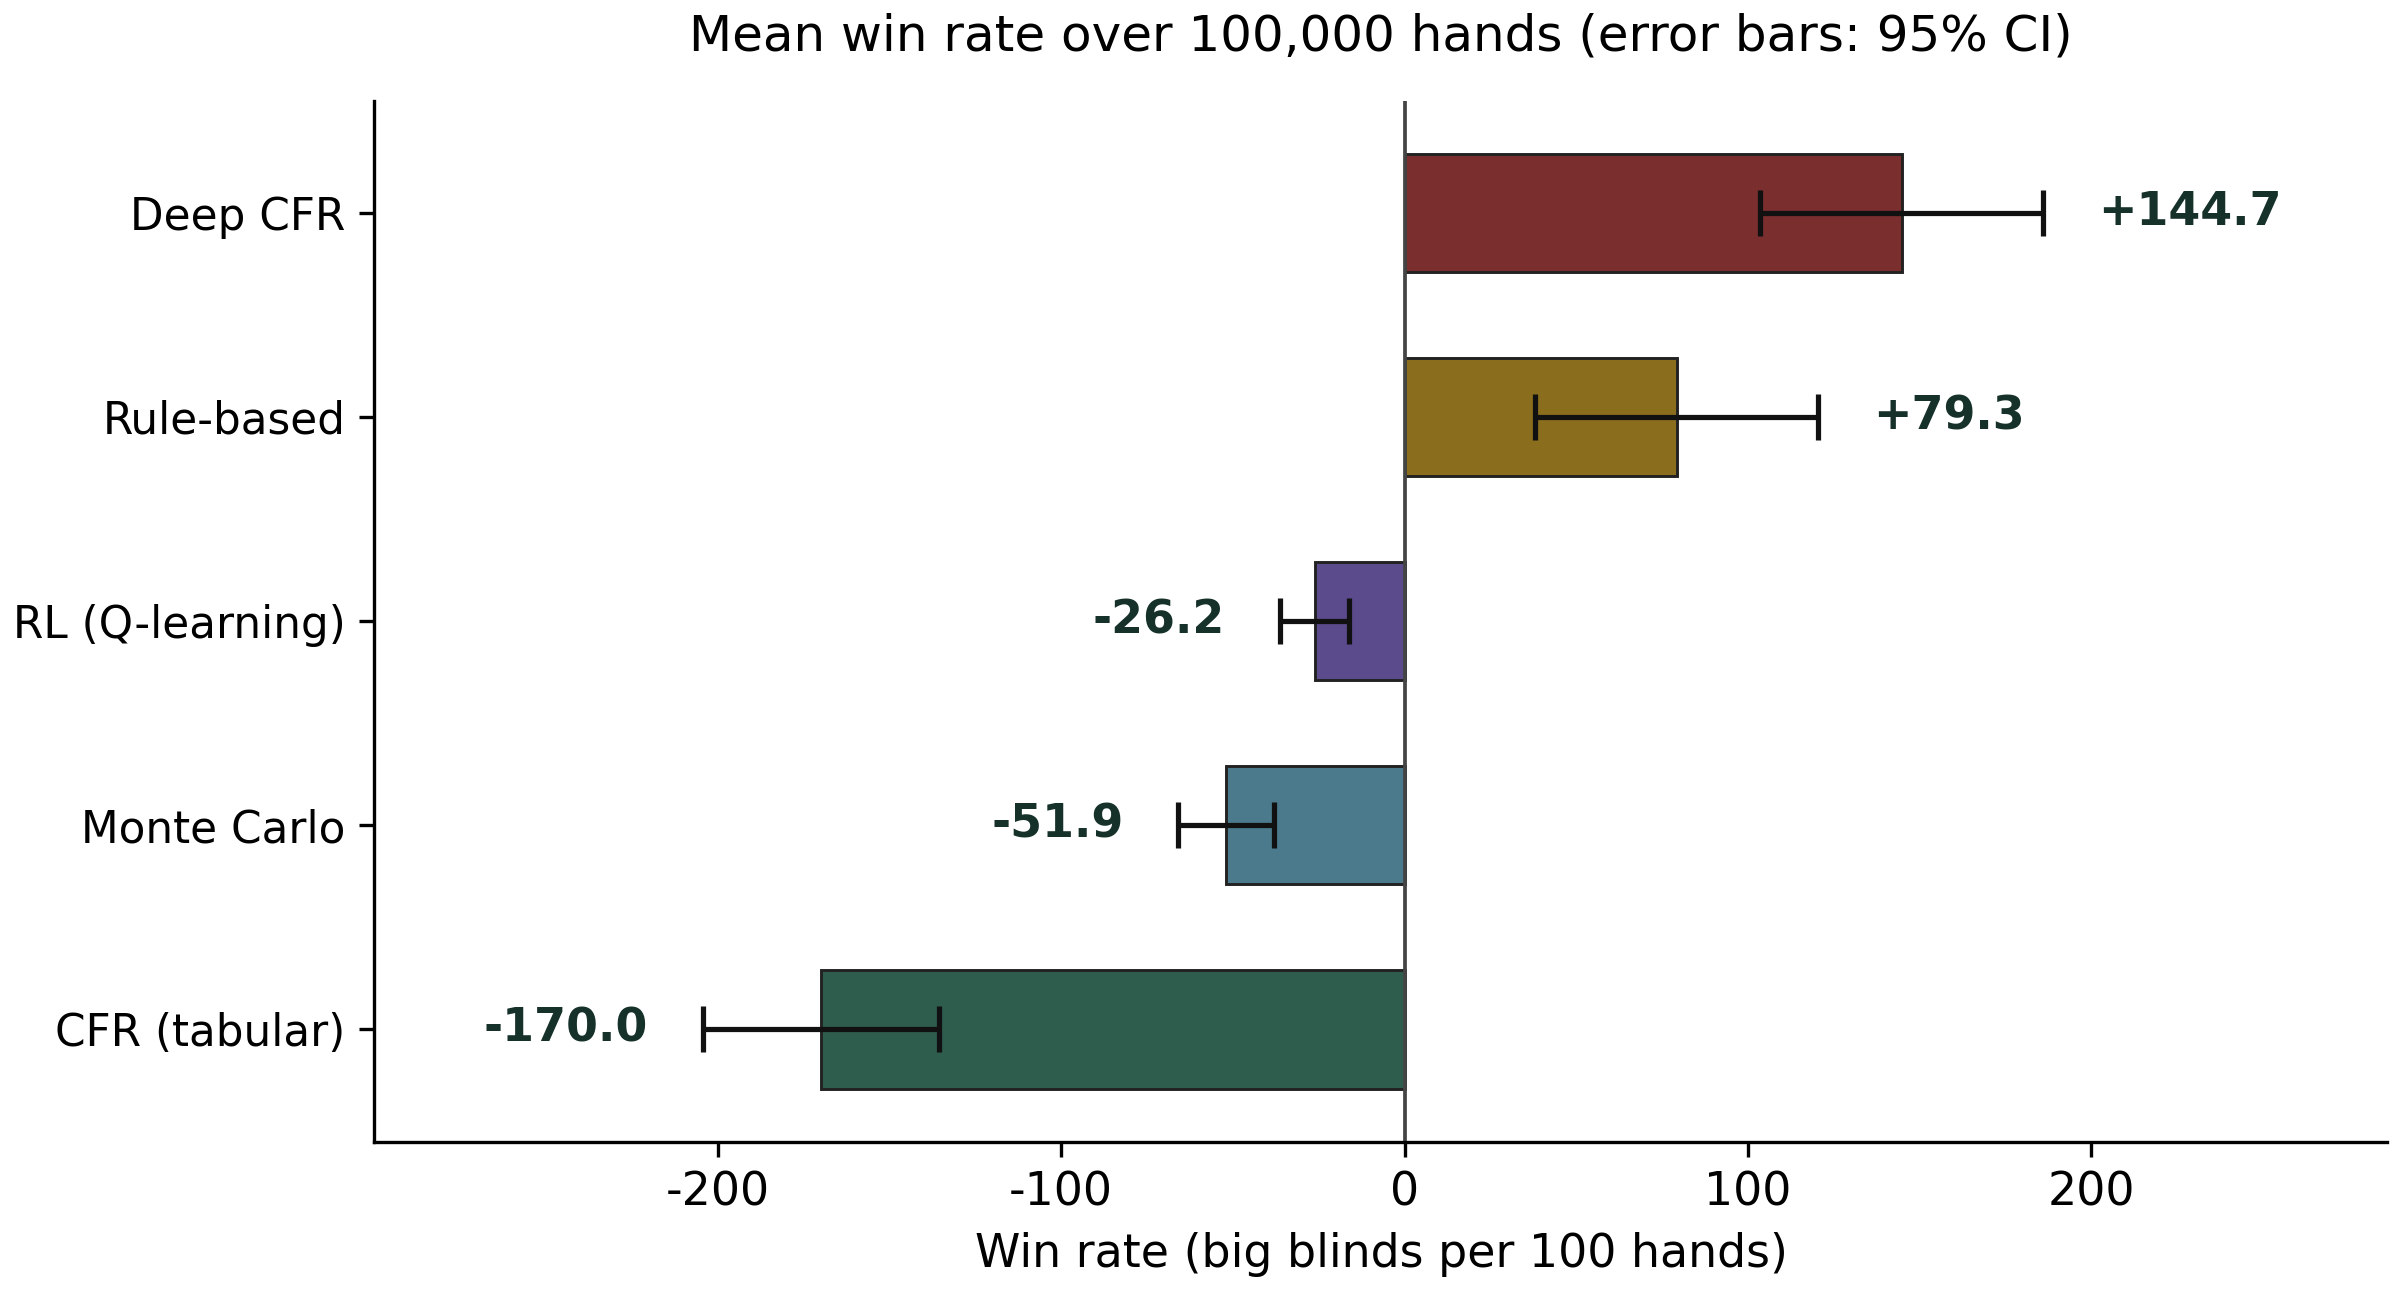
\includegraphics[width=0.94\textwidth]{figures/win_rates.png}
\caption{Mean win rate per paradigm over $100{,}000$ hands with $95\%$ confidence intervals. Every agent's win rate differs from zero significantly; the ordering is Deep CFR $>$ rule $>$ RL $>$ Monte Carlo $>$ tabular CFR, with the top and bottom agents separated by $11.5$ standard errors.}
\label{fig:winrates}
\end{figure}

Three headline facts emerge. First, \emph{every} win rate differs from zero significantly, and the pairwise separations are large: Deep CFR beats the tabular CFR agent by $314.7$\,bb/100 ($z = 11.5$) and beats the rule agent by $65.5$\,bb/100 ($z = 2.2$); the rule agent beats the tabular CFR agent by $249.3$\,bb/100 ($z = 9.1$). Second, the field is extraordinarily showdown-heavy: $64.0\%$ of hands reach showdown (against roughly $30\%$ in tight human six-max play), confirming that these agents neither fold enough nor steal enough. Third, per-hand volatility dwarfs the means---the standard deviation of a single hand's result ranges from $16$\,bb (RL) to $66$\,bb (rule, Deep CFR)---so the $10^{5}$-hand budget is what makes the ordering statistically decisive, precisely the regime \eqref{eq:handsneeded} anticipated.

\begin{figure}[htbp]
\centering
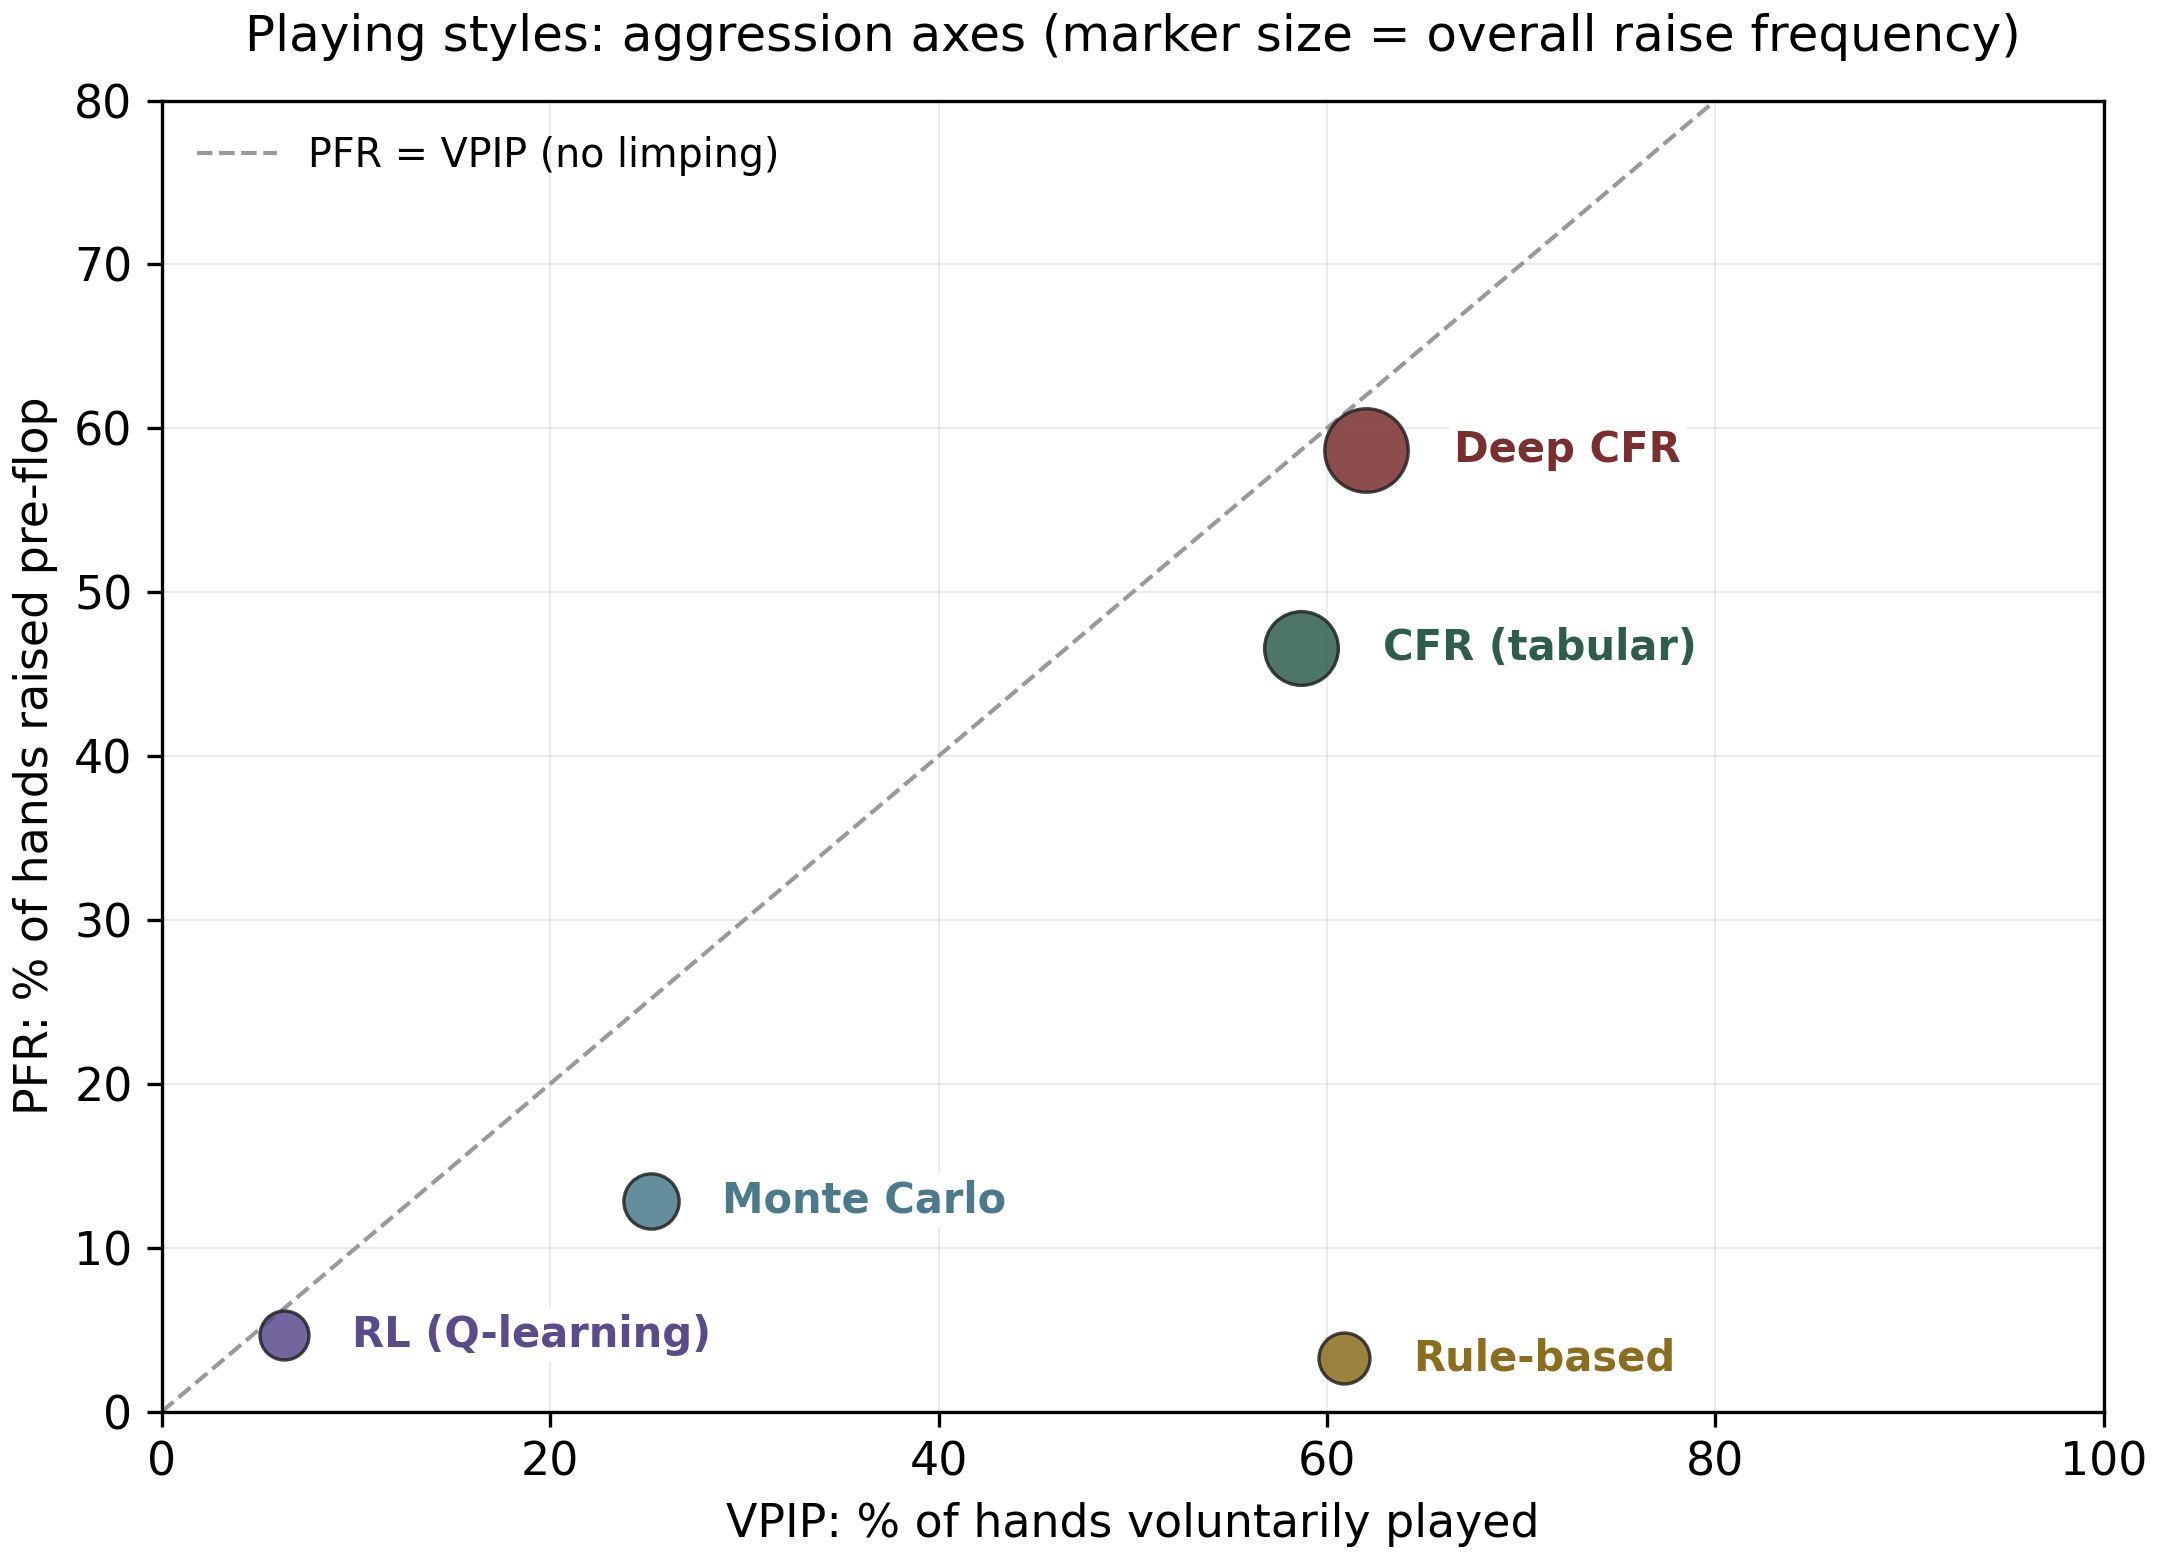
\includegraphics[width=0.86\textwidth]{figures/styles.png}
\caption{Style fingerprints in the VPIP--PFR plane (marker size proportional to overall raise frequency). The two CFR-family agents sit in the loose-aggressive quadrant with opposite fortunes; the rule agent is a loose-passive calling station; the RL agent learned an extreme nit profile; the Monte Carlo agent is tight and showdown-averse.}
\label{fig:styles}
\end{figure}

\subsection{Style analysis}

Figure~\ref{fig:styles} shows why the win-rate ordering is not a story about aggression alone. The two CFR-family agents occupy nearly the same loose-aggressive coordinates---CFR at (VPIP $58.6\%$, PFR $46.6\%$), Deep CFR at ($62.0\%$, $58.7\%$)---yet their win rates differ by $314.7$\,bb/100. The rule agent is their photographic negative: almost identical VPIP ($60.9\%$) but near-zero PFR ($3.2\%$), a textbook calling station that nonetheless wins $79.3$\,bb/100. The RL agent's learned policy is an extreme nit (VPIP $6.3\%$), folding everything except monsters---yet its showdown win rate when it does arrive ($51.4\%$) is second only to the Monte Carlo agent's $59.2\%$, and its losses are dominated by blind attrition. The Monte Carlo agent plays a tight-preflop, pot-odds-driven style that folds the flop to aggression (showdown frequency only $5.0\%$) and collects when it does continue ($59.2\%$ at showdown), a profile that is sound against balanced opponents and systematically wrong against a field that bets far too often.

\begin{figure}[htbp]
\centering
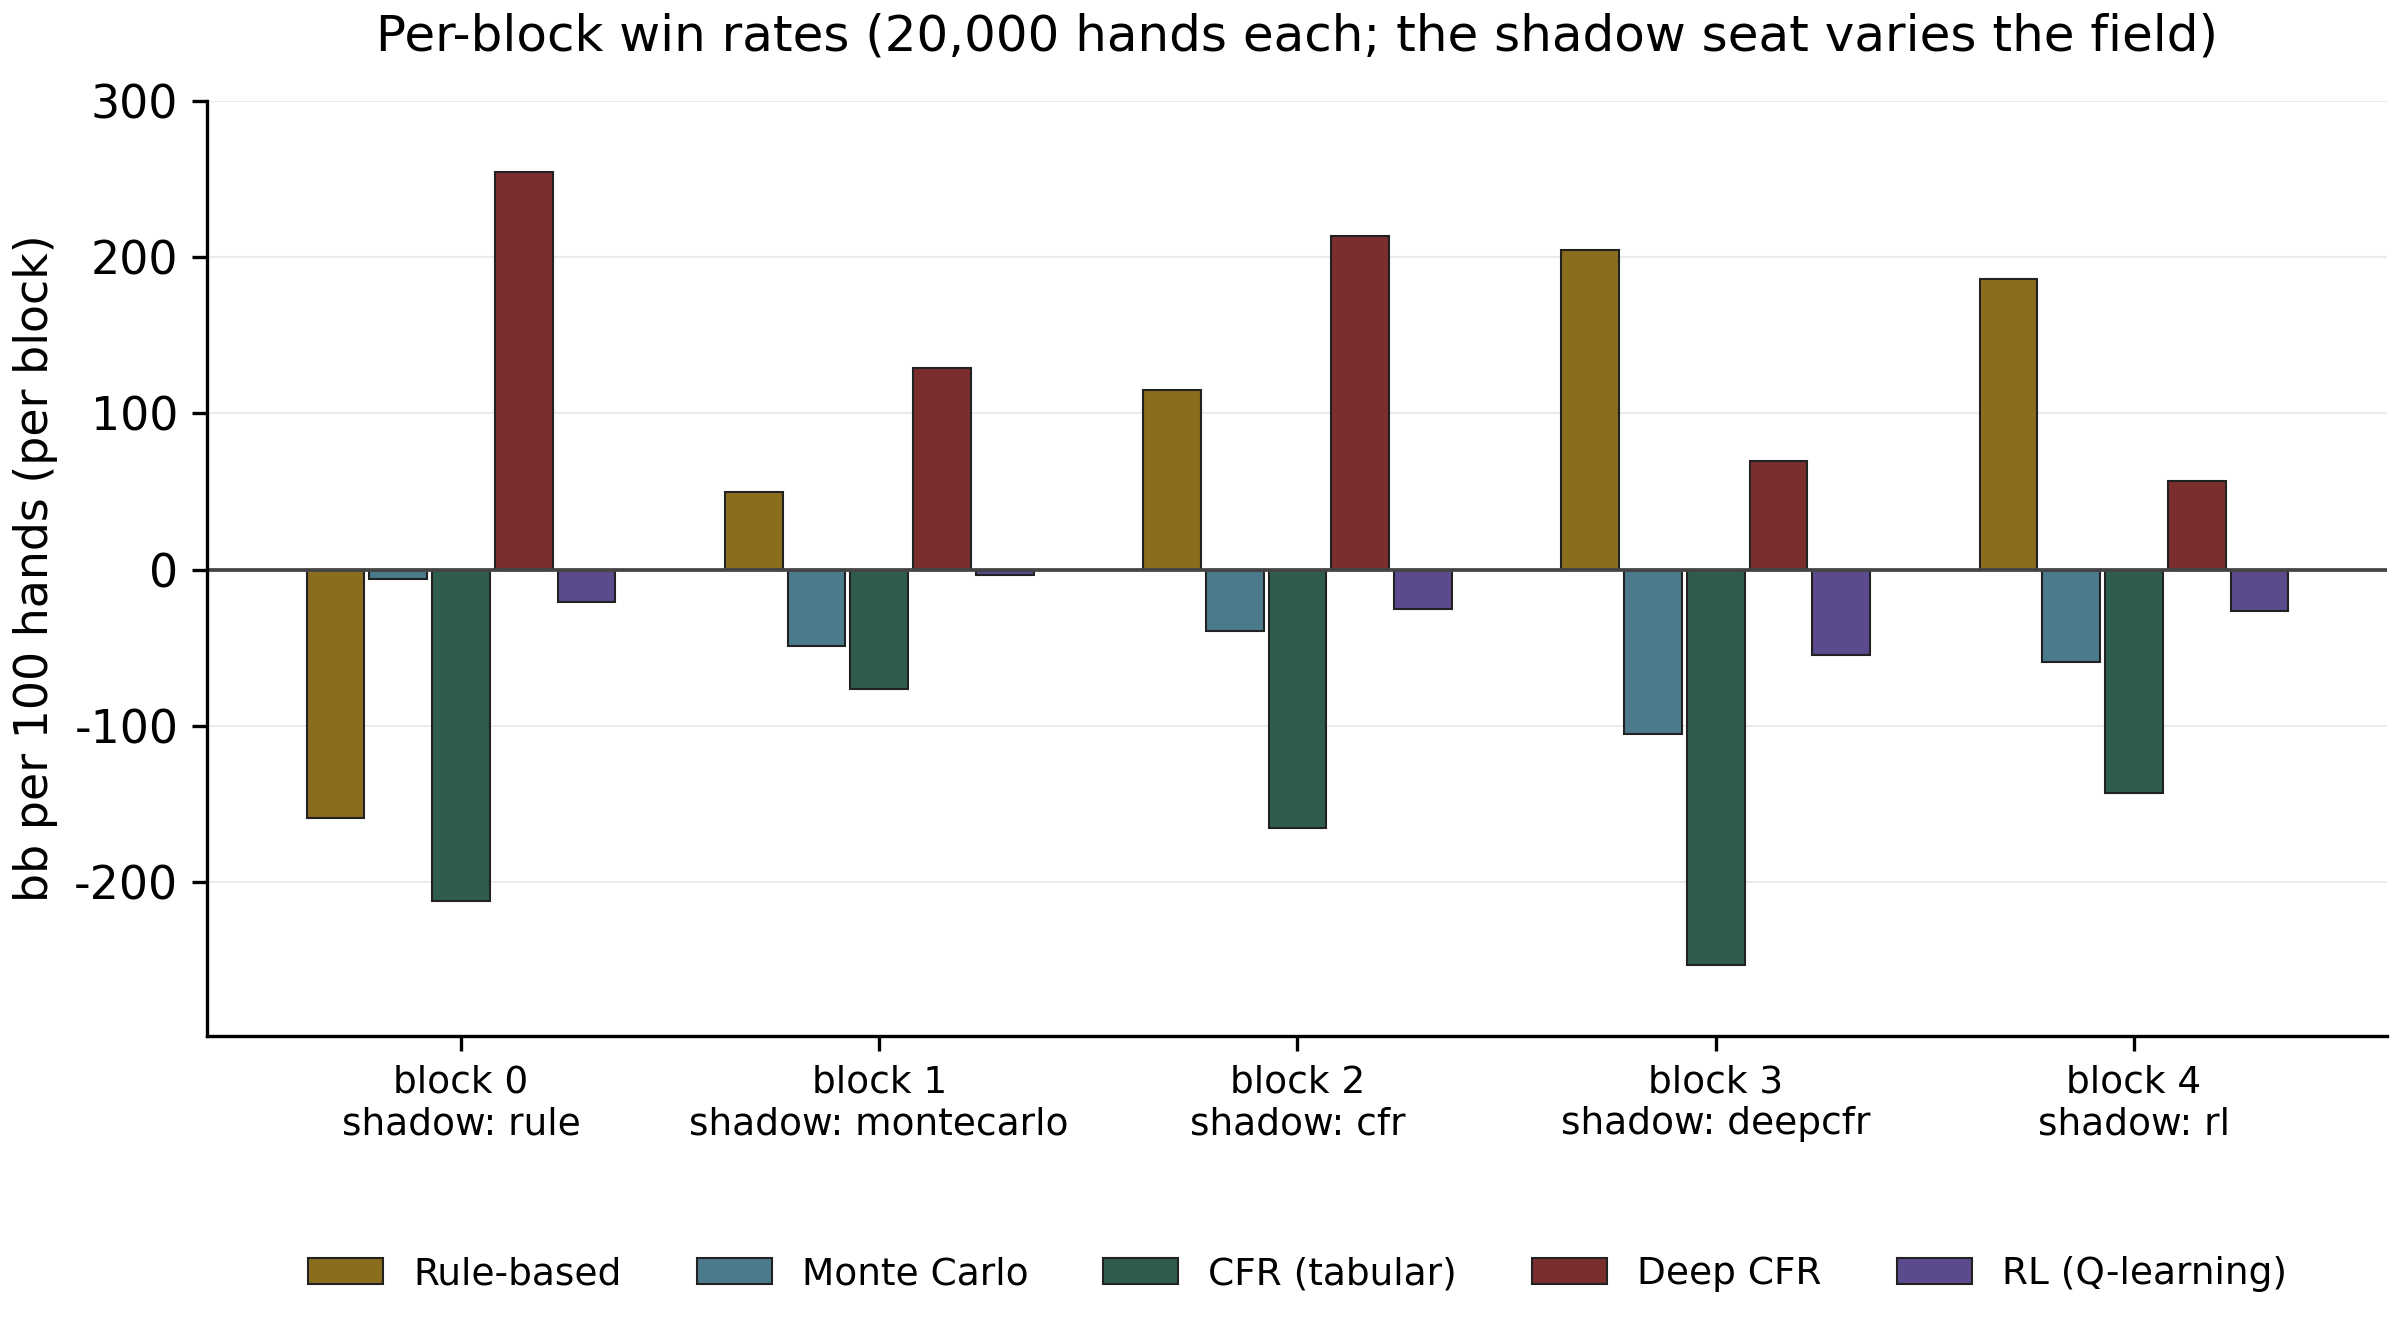
\includegraphics[width=0.94\textwidth]{figures/per_block.png}
\caption{Per-block win rates (20{,}000 hands per block). The shadow seat's identity (labelled below each block) changes the field composition; the ordering is largely stable across compositions, with Deep CFR the top or near-top earner everywhere and the tabular CFR agent losing in all five. The notable exception is the rule agent, whose result swings from $-159$\,bb/100 when the shadow duplicates itself to $+205$\,bb/100 when the shadow is the loose-aggressive Deep CFR---its calling-station style profits exactly when the extra opponent feeds it postflop calls---and the Monte Carlo / RL order flips in the block whose shadow duplicates the rule agent (with a second caller at the table, Monte Carlo's tight pot-odds play overtakes RL's blind-attrition losses).}
\label{fig:perblock}
\end{figure}

The per-block view (Figure~\ref{fig:perblock}) adds a robustness dimension: Deep CFR is the top or near-top earner in every field composition; the tabular CFR agent loses in all five; and the rule agent's two most profitable blocks are those whose shadow seats add either loose-aggressive opponents (Deep CFR, +$205$\,bb/100) or a second tight nit that surrenders blinds (RL, +$186$\,bb/100), while its worst block by far is the one whose shadow duplicates its own calling-station profile ($-159$\,bb/100).

\subsection{Interpretation: why did the equilibrium agent lose?}

The tabular CFR agent's $-170$\,bb/100 is the study's most instructive number, because it \emph{looks} like a refutation of Section~\ref{sec:cfr} and is in fact a layered confirmation of the theory's boundary conditions.

\emph{First, the multiplayer void.} CFR's guarantee---average strategy approaches an $\epsilon$-Nash equilibrium whose exploitability bound \eqref{eq:expl} protects the holder---is a two-player zero-sum statement (Theorem~\ref{thm:cfr} in conjunction with Section~\ref{sec:nash}). In a six-player game, regret minimisation against one's own self-play distribution converges toward a coarse correlated equilibrium-like object with \emph{no} safety property: Section~\ref{sec:nash}'s warning that multiplayer equilibrium is a robustness heuristic rather than an optimality certificate applies with full force to the blueprint we trained.

\emph{Second, the field calls.} Equilibrium aggression is priced for a rational responder: in Kuhn poker, the $1{:}3$ bluff--value ratio works because the opponent folds exactly often enough (Proposition~\ref{prop:kuhn}). This field does not fold---three of the five agents voluntarily play $58$--$62\%$ of hands and the table as a whole reaches showdown $64\%$ of the time---so bluffs at ``balanced'' frequencies become direct donations, and the blueprint's PFR of $46.6\%$ feeds pots to opponents who will pay to see rivers. The rule agent's profit is the mirror image of the same mispricing: a strategy that almost never bluffs and calls far too often is maximally punitive against an over-bluffing field, exactly as the Kuhn arithmetic predicts when the caller's folding rate deviates from equilibrium.

\emph{Third, the table is only partially converged.} Diagnostics on the trained blueprint quantify the practical gap between ``CFR in principle'' and ``this CFR run'': $18.7\%$ of the $13{,}873$ pooled strategy rows remain near-uniform (maximum action probability below $0.40$), and preflop rows---where most chips enter---are the least converged street (mean maximum probability $0.494$, against $0.64$--$0.68$ postflop). Whenever play reaches such a row, the agent acts near-uniformly over its legal actions: a sophisticated random player in exactly the spots that this field visits most. Months of compute close this gap in research systems; $25$ minutes does not.

\emph{Fourth, the sibling controls for the paradigm.} The decisive comparison is internal to the CFR family: same abstraction, same engine, same field, same training lineage---yet the tabular agent loses $170$\,bb/100 while the Deep CFR miniature wins $144.7$\,bb/100. The difference is not the learning principle but the \emph{representational fallback}: where the table has not been visited, it plays uniformly at random, whereas the advantage network outputs a smooth function of the state features and generalises to unvisited states. In a field this loose, coherence in the long tail of information sets is worth more than sharpness in the well-visited ones. We regard this as the study's cleanest lesson for practitioners: \emph{in small-budget settings, generalisation across information sets dominates table completeness.}

The RL agent's result completes the pattern. Its learned policy is a degenerate local optimum---folding all but $6\%$ of hands minimises variance against a training pool that included a random donor, and the terminal-only reward signal offered no gradient away from risk aversion. The policy was near-optimal \emph{against its pool} (training reward $+3.65$ chips per hand) and loses $-26.2$\,bb/100 against a different field: exploitation learned is field-specific, the guarantee asymmetry of Section~\ref{sec:nash} in miniature, produced by twenty seconds of self-play rather than by design.

\subsection{Threats to validity}

Four caveats bound the conclusions. (i) The study ranks \emph{implementations with these training budgets}, not paradigms: a months-scale blueprint, or a blueprint evaluated heads-up against a best responder, would occupy a different point in the space, and nothing here contradicts the exploitability guarantees that hold in two-player zero-sum settings. (ii) Field composition is endogenous: win rates are properties of the five-agent ecosystem, and adding one strong tight-aggressive agent would re-price every strategy in the table (the per-block swings of the rule agent make this visible). (iii) The shared abstraction, held fixed for comparability, is coarse (20 preflop and 10 postflop buckets, four abstract actions built from two raise sizes); all agents inherit its blind spots, and the Deep CFR agent's advantage is partly that its network interpolates across them. (iv) Statistical resolution, while sufficient for the headline separations (all $|z| \ge 2.2$; the top--bottom gap is $11.5\sigma$), cannot order agents within a few bb/100 of each other. With those boundaries stated, the study's summary is the one the theory foreshadowed: \emph{safety guarantees are field-independent but payoff-free against weak opponents; exploitation is field-relative and pays exactly as well as the field is exploitable; and representational generalisation decides who survives the long tail of states that training never reached.}

% !TeX root = ../main.tex
\section{Conclusion}\label{sec:conclusion}

This paper traced a single arc: from the arithmetic of cards to agents that play. The probabilistic core (Section~\ref{sec:probability}) is elementary but not optional---pot odds, the $1/\sqrt{n}$ wall of Monte Carlo estimation, and the variance computation behind \eqref{eq:handsneeded} set the boundaries within which every poker decision system must operate. The game-theoretic core (Sections~\ref{sec:gametheory}--\ref{sec:cfr}) supplies the conceptual shift that separates poker AI from classical game AI: in imperfect-information games, safety means equilibrium, equilibrium means mixed strategies, and mixed strategies mean accepting negative-EV actions (bluffs, calls that lose on average) as the premium paid for being unreadable. Kuhn poker compresses the entire lesson into twelve information sets, and its exact bluff--value arithmetic---one bluff per three value bets, matching the caller's pot odds to four decimal places---is the same arithmetic that governs no-limit bet sizing at any depth of stack.

The algorithmic ladder then formalised a trade-off that the experimental study made concrete. Rule-based expert systems (Section~\ref{sec:evaluation}) are transparent and fast but statically exploitable; Monte Carlo agents sharpen estimation while inheriting static decision thresholds; equilibrium blueprints computed by sampled CFR (Section~\ref{sec:cfr}) trade exploitability for unexploitability at the cost of an abstraction's fidelity; function approximation (Deep CFR) and trial-and-error learning (Q-learning, Section~\ref{sec:rl}) relax the tabular bottleneck in exchange for approximation error and non-stationarity hazards. The 100{,}000-hand tournament of Section~\ref{sec:experiments} measured where these trade-offs land when five paradigms share one table, under conditions---fixed stacks, rotating positions, seeded deals---designed so that observed differences are attributable to the agents rather than to seat luck, wealth compounding, or measurement artifacts.

Three engineering lessons generalise beyond poker. First, \emph{measurement discipline precedes interpretation}: our own investigation began with an apparent positional bias that dissolved under correct accounting, a reminder that in high-variance domains a plausible statistic unaccompanied by a variance calculation is indistinguishable from noise. Second, \emph{abstraction is not merely compression but a design language}: the choice of buckets, bet sizes, and betting-pattern keys encodes hypotheses about which strategic distinctions matter, and a shared abstraction is what makes controlled comparisons between paradigms meaningful at all. Third, \emph{guarantees and performance are different currencies}: the equilibrium-flavoured agents are certifiably hard to exploit within their abstract game, yet the tournament's winner is whichever agent's inductive biases happen to fit the field---a separation that mirrors the exploitation-versus-safety tension the theory predicts, and that future systems reconcile by combining both, as the superhuman programs do with blueprint equilibrium plus targeted real-time search.

The natural extensions of this work follow the field's trajectory: deeper stacks and finer action abstractions; exploitability measurement of the trained blueprints against best responses computed in the abstract game; end-to-end deep RL with NFSP-style averaging to place the learning paradigm on an equal representational footing with Deep CFR; and opponent modelling layered on top of equilibrium baselines, which is where commercial poker tools now concentrate their effort. The game has been kind to its students: each time the community declared the frontier closed---limit solved, heads-up solved, multiplayer superhuman---the remaining imperfections proved interesting enough to open the next one. Card probabilities, regret, and reinforcement learning will keep finding work at that frontier.


% !TeX root = ../main.tex
\begin{thebibliography}{25}
\small
\setlength{\itemsep}{2pt}

\bibitem{billings2002challenge}
D.~Billings, A.~Davidson, J.~Schaeffer, and D.~Szafron.
\newblock The challenge of poker.
\newblock \emph{Artificial Intelligence}, 134(1--2):201--250, 2002.

\bibitem{bowling2015ceph}
M.~Bowling, N.~Burch, M.~Johanson, and O.~Tammelin.
\newblock Heads-up limit hold'em poker is solved.
\newblock \emph{Science}, 347(6218):145--149, 2015.

\bibitem{brown2017libratus}
N.~Brown and T.~Sandholm.
\newblock Superhuman AI for heads-up no-limit poker: Libratus beats top professionals.
\newblock \emph{Science}, 359(6374):418--424, 2018.

\bibitem{brown2018depth}
N.~Brown and T.~Sandholm.
\newblock Depth-limited solving for imperfect-information games.
\newblock In \emph{Advances in Neural Information Processing Systems 31}, pages 7662--7672, 2018.

\bibitem{brown2019pluribus}
N.~Brown and T.~Sandholm.
\newblock Superhuman AI for multiplayer poker.
\newblock \emph{Science}, 365(6456):885--890, 2019.

\bibitem{brown2019deep}
N.~Brown, A.~Lerer, S.~Gross, and T.~Sandholm.
\newblock Deep counterfactual regret minimization.
\newblock In \emph{Proceedings of the 36th International Conference on Machine Learning (ICML)}, pages 793--802, 2019.

\bibitem{cesabianchi2006prediction}
N.~Cesa-Bianchi and G.~Lugosi.
\newblock \emph{Prediction, Learning, and Games}.
\newblock Cambridge University Press, 2006.

\bibitem{heinrich2016deep}
J.~Heinrich and D.~Silver.
\newblock Deep reinforcement learning from self-play in imperfect-information games.
\newblock \emph{arXiv preprint arXiv:1603.01121}, 2016.

\bibitem{kelly1956new}
J.~L.~Kelly, Jr.
\newblock A new interpretation of information rate.
\newblock \emph{Bell System Technical Journal}, 35(4):917--926, 1956.

\bibitem{kuhn1953extensive}
H.~W.~Kuhn.
\newblock Extensive games and the problem of information.
\newblock In \emph{Contributions to the Theory of Games II}, Annals of Mathematics Studies 28, pages 193--216. Princeton University Press, 1953.

\bibitem{lanctot2009monte}
M.~Lanctot, K.~Waugh, M.~Zinkevich, and M.~Bowling.
\newblock Monte Carlo sampling for regret minimization in extensive games.
\newblock In \emph{Advances in Neural Information Processing Systems 22}, pages 1078--1086, 2009.

\bibitem{moravcik2017deepstack}
M.~Morav\v{c}\'ik, M.~Schmid, N.~Burch, V.~Lis\'y, D.~Morrill, N.~Bard, T.~Davis, K.~Waugh, M.~Johanson, and M.~Bowling.
\newblock DeepStack: Expert-level artificial intelligence in heads-up no-limit poker.
\newblock \emph{Science}, 356(6337):508--513, 2017.

\bibitem{nash1950equilibrium}
J.~F.~Nash.
\newblock Equilibrium points in $n$-person games.
\newblock \emph{Proceedings of the National Academy of Sciences}, 36(1):48--49, 1950.

\bibitem{robinson1951iterative}
J.~Robinson.
\newblock An iterative method of solving a game.
\newblock \emph{Annals of Mathematics}, 54(2):296--301, 1951.

\bibitem{sandholm2015abstraction}
T.~Sandholm.
\newblock Abstraction for solving imperfect-information games.
\newblock In \emph{Proceedings of the 29th AAAI Conference on Artificial Intelligence}, pages 4121--4126, 2015.

\bibitem{schnizlein2012card}
D.~Schnizlein, M.~Bowling, and D.~Szafron.
\newblock Probabilistic card abstraction for equilibrium analysis in poker.
\newblock In \emph{Proceedings of the 26th AAAI Conference on Artificial Intelligence}, pages 1508--1514, 2012.

\bibitem{silver2017alphagozero}
D.~Silver, J.~Schrittwieser, K.~Simonyan, et al.
\newblock Mastering the game of Go without human knowledge.
\newblock \emph{Nature}, 550(7676):354--359, 2017.

\bibitem{sutton2018rl}
R.~S.~Sutton and A.~G.~Barto.
\newblock \emph{Reinforcement Learning: An Introduction}.
\newblock MIT Press, second edition, 2018.

\bibitem{tammelin2015cfrplus}
O.~Tammelin.
\newblock Solving large imperfect information games using CFR$^{+}$.
\newblock \emph{arXiv preprint arXiv:1407.5042}, 2014.

\bibitem{tesauro1995td}
G.~Tesauro.
\newblock Temporal difference learning and TD-Gammon.
\newblock \emph{Communications of the ACM}, 38(3):58--68, 1995.

\bibitem{waugh2009abstraction}
K.~Waugh, D.~Schnizlein, M.~Bowling, and D.~Szafron.
\newblock Abstraction pathologies in extensive games.
\newblock In \emph{Proceedings of the 8th International Joint Conference on Autonomous Agents and Multiagent Systems (AAMAS)}, pages 781--788, 2009.

\bibitem{watkins1992q}
C.~J.~C.~H.~Watkins and P.~Dayan.
\newblock Q-learning.
\newblock \emph{Machine Learning}, 8(3--4):279--292, 1992.

\bibitem{zinkevich2007regret}
M.~Zinkevich, M.~Johanson, M.~Bowling, and C.~Piccione.
\newblock Regret minimization in games with incomplete information.
\newblock In \emph{Advances in Neural Information Processing Systems 20}, pages 1729--1736, 2008.

\end{thebibliography}


\end{document}
